\newpage
\setcounter{page}{1}
%\onehalfspacing
\doublespacing
\section{Review of the literature}

\subsection{Introduction}
	
	Viruses are seemingly simple in comparison to organisms that they infect and consist of just a genome, structural proteins and sometimes a lipid bilayer envelope. Because of this simplicity they have very limited capacity to encode factors essential for their own replication and are fully dependent on host cells. Viruses are obligate parasites of cells and have evolved multiple strategies to interact with the cell at each step of viral life cycle. For this, specific viral proteins interact with the numerous host factors and subvert cellular processes to fulfill the needs of virus replication. 
			
	The initial interaction event between the virus and a susceptible cell occurs when viral receptor-binding proteins recognize cellular proteins, carbohydrates or lipids exposed on the cell surface \parencite{Grove2011}. Viruses enter the cell via non-endocytic or endocytic routes, which often require interaction with cellular factors, such as clathrin-coated vesicle components \parencite{Dimitrov2004, Yamauchi2013}. Interaction with the cellular cytoskeleton is widely used by viruses to accelerate and direct their antero- and retrograde transport through the crowded intra-cellular environment \parencite{Ploubidou2001}. Uncoating and release of viral genomes is often triggered by interaction with specific cellular proteins \parencite{Suomalainen2013, Haywood2010}. Furthermore, viruses that replicate in the nucleus translocate their components to the nucleus in an active way which requires binding to the proteins of nuclear pore complex \parencite{Kobiler2012}.
				
	Independently on whether they encode own their RNA polymerase or use the cellular enzyme, complex interactions with the cellular transcription machinery ensure effective synthesis of viral mRNA. For example, poliovirus and \gls{RVFV}, which use their own enzymes for RNA synthesis both shut down host transcription, which is not essential for viral replication \parencite{Kundu2005, LeMay2004}. In contrast, the viruses that require host transcription machinery, for example \gls{HSV}, set up regulatory interactions with cellular transcription factors to support their own DNA synthesis \parencite{Wysocka2003}.

	Furthermore, being restricted in their encoding capacity viruses lack their own functional translation machinery and fully rely on host protein synthesis \parencite{Walsh2011}. Even \textit{Pandoravirus salinus} with the biggest known viral genomes of 2.77 \gls{Mb} encodes only few required translation factors remaining dependent on protein synthesis of its \textit{Acantamoeba} host \parencite{Philippe2013}. Viruses target the cellular translational machinery to secure preferential translation of viral transcripts or to shut off host translation when it is not required. For instance, \gls{VSV} utilizes specific 3' structures on its mRNA and also interacts with the ribosome to secure preferential synthesis of viral proteins \parencite{Whitlow2006, Lee2013}. Viruses further utilize cellular processes for transport of their components or assembled virions and for escape from the cell \parencite{Bartenschlager2011, Lyles2013}. Thus, HIV-1 usurps cellular endosomal sorting complexes required for transport pathway for its effective budding \parencite{Morita2011}, whereas adenoviruses induce autophagy to enable cell lysis and viral exit \parencite{Jiang2011}.
	
	The cells vertebrates, many invertebrates and plants respond to infection with robust induction of innate immune responses and no successful virus replication would be possible without control over these responses. For this, viruses have evolved a multitude of approaches to counteract their recognition by cellular detectors, \parencite{Zinzula2013}, subvert signal transduction, prevent activation of antiviral genes \parencite{Short2009}, and, when necessary, limit apoptosis \parencite{Galluzzi2008}.
	
	The number of viral strategies to interact with the host cell is overwhelming. Although we were able to deduce the basic strategies of viral life cycle from the nature of viral genomes already in 1971 \parencite{Baltimore1971}, the exact mechanisms of viral replication are so diverse and complicated that we are still striving to understand them. We study virus-host interactions largely in our attempts to improve surveillance of pathogenic viruses, search for antivirals and vaccine development \parencite{Webby2003, Schwegmann2008}. We also study virus-host interactions as viruses have proven many times to be valuable tools for understanding cell functions, from the initial discovery of DNA as genetic material \parencite{Hershey1952}, up to recent advances in tackling complex processes such as endocytosis \parencite{Pelkmans2003}. Finally, understanding virus-host interactions brings us novel applicable tools widely used in biotechnology, such as viral vectors for gene transfer \parencite{Vannucci2013} or baculovirus systems for heterologous protein production \parencite{VanOers2011}. Although a great deal of mechanisms have been already discovered, the amount of information that we get now is growing exponentially and majority of discoveries is perhaps still ahead. 
		
\subsection{Influenza A virus: an overview}
	
	This work is dedicated to influenza A virus, a member of the \textit{Orthomyxoviridae} family. Influenza A viruses are commonly classified based on their surface antigens \gls{HA} and \gls{NA}. All 16 subtypes of \gls{HA} and all 9 subtypes of \gls{NA} are found in wild birds which, apparently, represent the natural reservoir of influenza A virus \parencite{Stallknecht2007}. However, certain viral subtypes can also infect domesticated birds and multiple species of mammals, including humans. Whereas influenza A virus is asymptomatic in its natural hosts, it can cause mild to severe intestinal infections in poultry and asymptomatic to severe respiratory infections in mammals \parencite{Webster1992a}. 
	
	Although the first human influenza A virus was isolated in 1933 \parencite{Smith1933} and one of the first well-publicized influenza A pandemics occurred in 1918 \parencite{Taubenberger1997}, numerous records indicate that humankind has been facing influenza epidemics and probably also pandemics for at least several centuries \parencite{Potter2001}. There is molecular evidence that influenza A \gls{HA} subtypes 1, 2, 3, 5, 7 and 9 can infect humans, but the  majority of human influenza A infections are caused by H1 and H3 viruses.
	
	Circulating strains of influenza A cause seasonal infections in humans. In most countries these infections result in annual epidemics which affect up to 10 \% of the population worldwide and result in up to $500,000$ deaths (\hyperlink{www.who.in}{World Health Organization}). In addition to these annual epidemics, global pandemics can occur when humans are infected with viruses to which they are immunologicaly na\"{i}ve. Although influenza A pandemics are relatively rare events, humankind has faced three major pandemics in the XX century and already one in the twenty-first \parencite{Lagace-Wiens2010, Fineberg2014}.  Whereas the mortality of seasonal influenza is modest, the mortality of pandemic influenza is unpredictable and can vary: for example, during the H1N1 pandemic in 2009 it was below 0.5~\%, but during the H5N1 pandemic in 1997 it reached 60~\% \parencite{Forrest2010, Noah2013}. In addition to annual influenza-related deaths, the virus imposes an enormous economic burden both to health care and to agriculture \parencite{Szucs1999, Noah2013}. 
	
	Influenza A virus genome is composed of eight \gls{ssRNA} molecules of negative polarity  \parencite{Palese1977}. It is replicated with the viral \gls{rdrp} which is error-prone and produces between $1.5$ and $7.5\times10^{-5}$ misincorporations per nucleotide. Because \gls{rdrp} also lacks proofreading activity these misincorporations cannot be repaired and on average one mutation appears the viral genome after each replication cycle \parencite{Drake1993, Parvin1986}. The gradual evolution of influenza A viruses due to frequent mutations in viral proteins is referred to as antigenic drift. In addition, the viral genomic segments can reassort during the co-infection of the same cell with distinct influenza A viruses and give rise to progeny virions that contain segments derived from both ``parental'' viruses \parencite{McGeoch1976, Desselberger1978}. Such major changes in the virus are referred to as antigenic shift. Antigenic drift and antigenic shift are the key drivers of viral evolution \parencite{Forrest2010}. Antigenic drift limits efficacy of vaccines and  antivirals and antigenic shift imposes constant risk for new pandemics. Thus, improvement of options to control influenza are needed. These efforts require careful virus surveillance, vaccine development and search for antivirals with novel mechanisms of action. They are impossible without a comprehensive understanding of influenza A virus-host interactions.
	
\subsection{Influenza A virus organization and replication cycle}

	Influenza A virions are pleiomorphic, i.e. their shapes are not uniform and can be spherical, kidney- or rod-shaped with an average size of 100--150 nm \parencite{Fujiyoshi1994}. The outer shell of the virion is composed of the host-derived lipid bilayer in which viral \gls{HA}, \gls{NA} and \gls{M2} are incorporated. This shell is underlined with the viral \gls{M1} \parencite{Harris2006}. Each virion encompasses eight genomic RNA segments packed \glspl{vRNP}~--- supercoiled ring-like structures in which paired 5' and 3' ends of the viral RNA are associated with heterotrimetic viral polymerase complex and the rest of the RNA is densely covered with viral \gls{NP} \parencite{Arranz2012}. In the virion the \glspl{vRNP} are associated with the \gls{M1} protein \parencite{Rees1982, Ye1999}. Eight genes of all influenza A viruses encode 10 essential viral proteins: \gls{HA}, \gls{NA}, \gls{M1}, \gls{M2}, \gls{NP}, \gls{PB1}, \gls{PB2}, \gls{PA}, \gls{NS1}, and \gls{NEP} \parencite{Lamb1983}. In addition, some influenza A strains may encode accessory proteins PB1-F2, PB1-N40, PA-X, PA-155 and PA-182. Whereas \gls{HA}, \gls{NA}, \gls{M1}, \gls{M2}, \gls{NP}, \gls{PB1}, \gls{PB2}, \gls{PA} and \gls{NEP} are structural components of viral particle, \gls{NS1}, PB1-F2, PB1-N40, PA-X, PA-155 and PA-182 are considered to be non-structural and are involved in regulation of virus-host interactions \parencite{Chen2001,Hale2008b,Wise2009,Jagger2012,Muramoto2013}.
	
	Influenza A replication cycle begins when the viral \gls{HA} binds to the specific virus receptor on cell surface. The key, but possibly not the only receptors for influenza A virus are sialic acids linked to cellular surface glycoproteins or glycolipids \parencite{Skehel2000, Stray2000, Martin1998}. \gls{HA} molecules of avian influenza A viruses recognize $\alpha$-2,3-linked sialic acids and \gls{HA} of human influenza A viruses recognize $\alpha$-2,6-linked sialic acids \parencite{Connor1994, VanRiel2010}. \gls{HA} recognition of specific sialic acids to a large extent determines viral host specificity. After receptor binding the viruses are endocytosed via clathrin-dependent or clathrin- and caveolin-independent routes and are transferred towards the perinuclear space in endosomes \parencite{Dourmashkin1974, Matlin1981, Sieczkarski2002, Lakadamyali2003}. Acidification of late endosomes in perinuclear space triggers two essential events that allow virus uncoating and delivery of \gls{vRNP}s to the cytoplasm. First, low pH mediates the conformational change in the \gls{HA} and enables fusion of viral and endosomal membranes \parencite{Carr1993}. Second, acidification of the virus interior leads to dissociation of \glspl{vRNP} from \gls{M1} which is a prerequisite for their import to the nucleus, a site of influenza A replication \parencite{Bui1996, Stauffer2014}. 
	
	In the nucleus the \glspl{vRNA} are transcribed \textit{in cis} by the viral polymerase associated with the \gls{vRNP} \parencite{Moeller2012}. Synthesis of viral mRNA is initiated using 10--13 nucleotide long primers with \gls{5meG} \parencite{Beaton1981, Plotch1981a}. These primers are stolen from cellular mRNAs during ``cap-snatching'' when \gls{5meG} cap structures on host mRNAs are recognized and bound by \gls{PB2} subunit of viral polymerase \parencite{Guilligay2008} and further endonucleolytically cleaved by viral \gls{PB1} and \gls{PA} \parencite{Li2001, Dias2009, Yuan2009}. The ``snatched'' \gls{5meG}-caps also provide 3'-OH ends for viral mRNA chain elongation by \gls{PB1} \parencite{Poch1989}. The synthesis of viral mRNA ends after reiterative copying of short uridine stretches located at the 5' end of vRNA and the resulting viral mRNA contains 150--200 adenine bases at its 3' end \parencite{Plotch1977, Robertson1981d, Poon1999}. Cap-containing polyadenylated viral mRNAs are structurally indistinguishable from cellular transcripts. They are exported from the nucleus via the cellular RNA export machinery and are translated in the cytoplasm \parencite{Chen2000}. Many of the synthesized viral proteins  shuttle back to the nucleus to facilitate production of new \gls{vRNP}s and their export to the cytoplasm \parencite{Greenspan1988, Neumann1997, Huet2010, Wang2013}. 
	
	Replication of influenza A viral genomes occurs through two steps. First, \gls{cRNP}s containing positive single-stranded cRNA are produced. Next, these \gls{cRNP}s serve as templates for production of progeny \gls{vRNP} \parencite{Elton2005}. In contrast to mRNA, the synthesis of both cRNA and vRNA is carried out \textit{in trans} by the free viral polymerase available in the nucleus after synthesis and import of new viral proteins \parencite{Jorba2009, Moeller2012}. Moreover, initiation of both cRNA and vRNA synthesis does not require cell- or virus-derived primers and occurs \textit{de novo} resulting in the presence of triphosphates at their 5' ends \parencite{Hay1982, Zhang2010}. The progeny \gls{vRNP}s are assembled in the nucleus and contain exact copies of parental vRNA, a single viral polymerase and multiple copies of \gls{NP}. They can be transcribed and later exported from the nucleus for virion assembly \parencite{Resa-Infante2011}. 
	
	Virion assembly and budding occurs at the cellular plasma membrane and requires transport of essential components of progeny virions to the site of assembly. The \gls{vRNP}s in a complex with \gls{M1} and \gls{NEP} are exported from the nucleus via cellular Crm1/exportin-1 pathway and then are transported to the site of budding via cellular microtubules \parencite{Akarsu2003, Momose2007, Kawaguchi2012}. Viral envelope proteins (\gls{HA}, \gls{NA} and \gls{M1}) obtain specific sorting signals for their targeting to the budding site \parencite{Hughey1992, Kundu1996, Tall2003} and are transported there through the Golgi network \parencite{Daniels-Holgate1989}. The virion assembly is localized to specific  cholesterol- and sphingolipid-enriched regions of plasma membrane referred to as lipid rafts \parencite{Scheiffele1999}. The budding requires \gls{M1}, \gls{HA} for initiation of cellular membrane curvature, coordinated interaction of \gls{M1} and \gls{vRNP}s for packaging of viral genomes and \gls{M2} for bud scission \parencite{Nayak2009a, Rossman2011}. After virion assembly and bud formation \gls{NA} cleaves the sialic acids off the cellular surface releasing new virions that can initiate another infection cycle \parencite{Barman2004}.

	
	\subsection{Host factors involved in IAV replication cycle}
	
	Because of the limited capacity of influenza A virus to encode its own proteins, its effective replication relies on cellular factors. A large number of such factors have been recently identified using yeast two-hybrid assay, genome-wide RNAi screening, and proteomic approaches \parencite{Mayer2007, Brass2009, Shapira2009, Hao2008, Karlas2010, Konig2010, Shaw2011, Song2011}. At least 128 of them were identified in two or more screens simultaneously. Functional clustering of these factors revealed their involvement in essentially all stages of viral replication \parencite{Watanabe2010}. A scheme summarizing host factors involved in different steps influenza A replication cycle is present on Figure \ref{fig:cycle}.
	
	Thus, the clathrin-mediated endocytosis of influenza A requires cellular clathrin epsin-1 \parencite{Chen2008a} and efficient endosomal transport depends on cellular GTPases Rab5 and Rab7 \parencite{Sieczkarski2003}. Fusion of viral and endosomal membranes is dependent on \gls{vATPase} that acidifies endosomal interior and several subunits of this macromolecular complex have been identified as host factors required for influenza A replication \parencite{Watanabe2010}. 
	
	Nuclear import of \gls{vRNP}s occurs in an active way and requires the interaction of \gls{NP} with importin $\alpha$1 or importin $\alpha$5 \parencite{Cros2005}. Although influenza A RNAs are transcribed by its own \gls{rdrp}, it interacts with cellular DNA-dependent RNA polymerase II presumably to facilitate cap snatching \parencite{Engelhardt2005}. Furthermore, influenza A utilizes cellular splicing machinery to process its mRNAs derived from segments 7 and 8 \parencite{Dubois2014} and cellular nuclear export machinery to deliver its transcripts to the cytoplasm \parencite{York2013}. As the virus encodes none of the translation machinery components, its protein synthesis completely depends on the host translation machinery and the efficacy of viral protein production is secured via the tight interaction between viral \gls{NS1} and cellular translation factors \parencite{DelaLuna1995, Burgui2003, Aragon2000}.
	
	\begin{figure}[h!]
				\centering
				\fbox{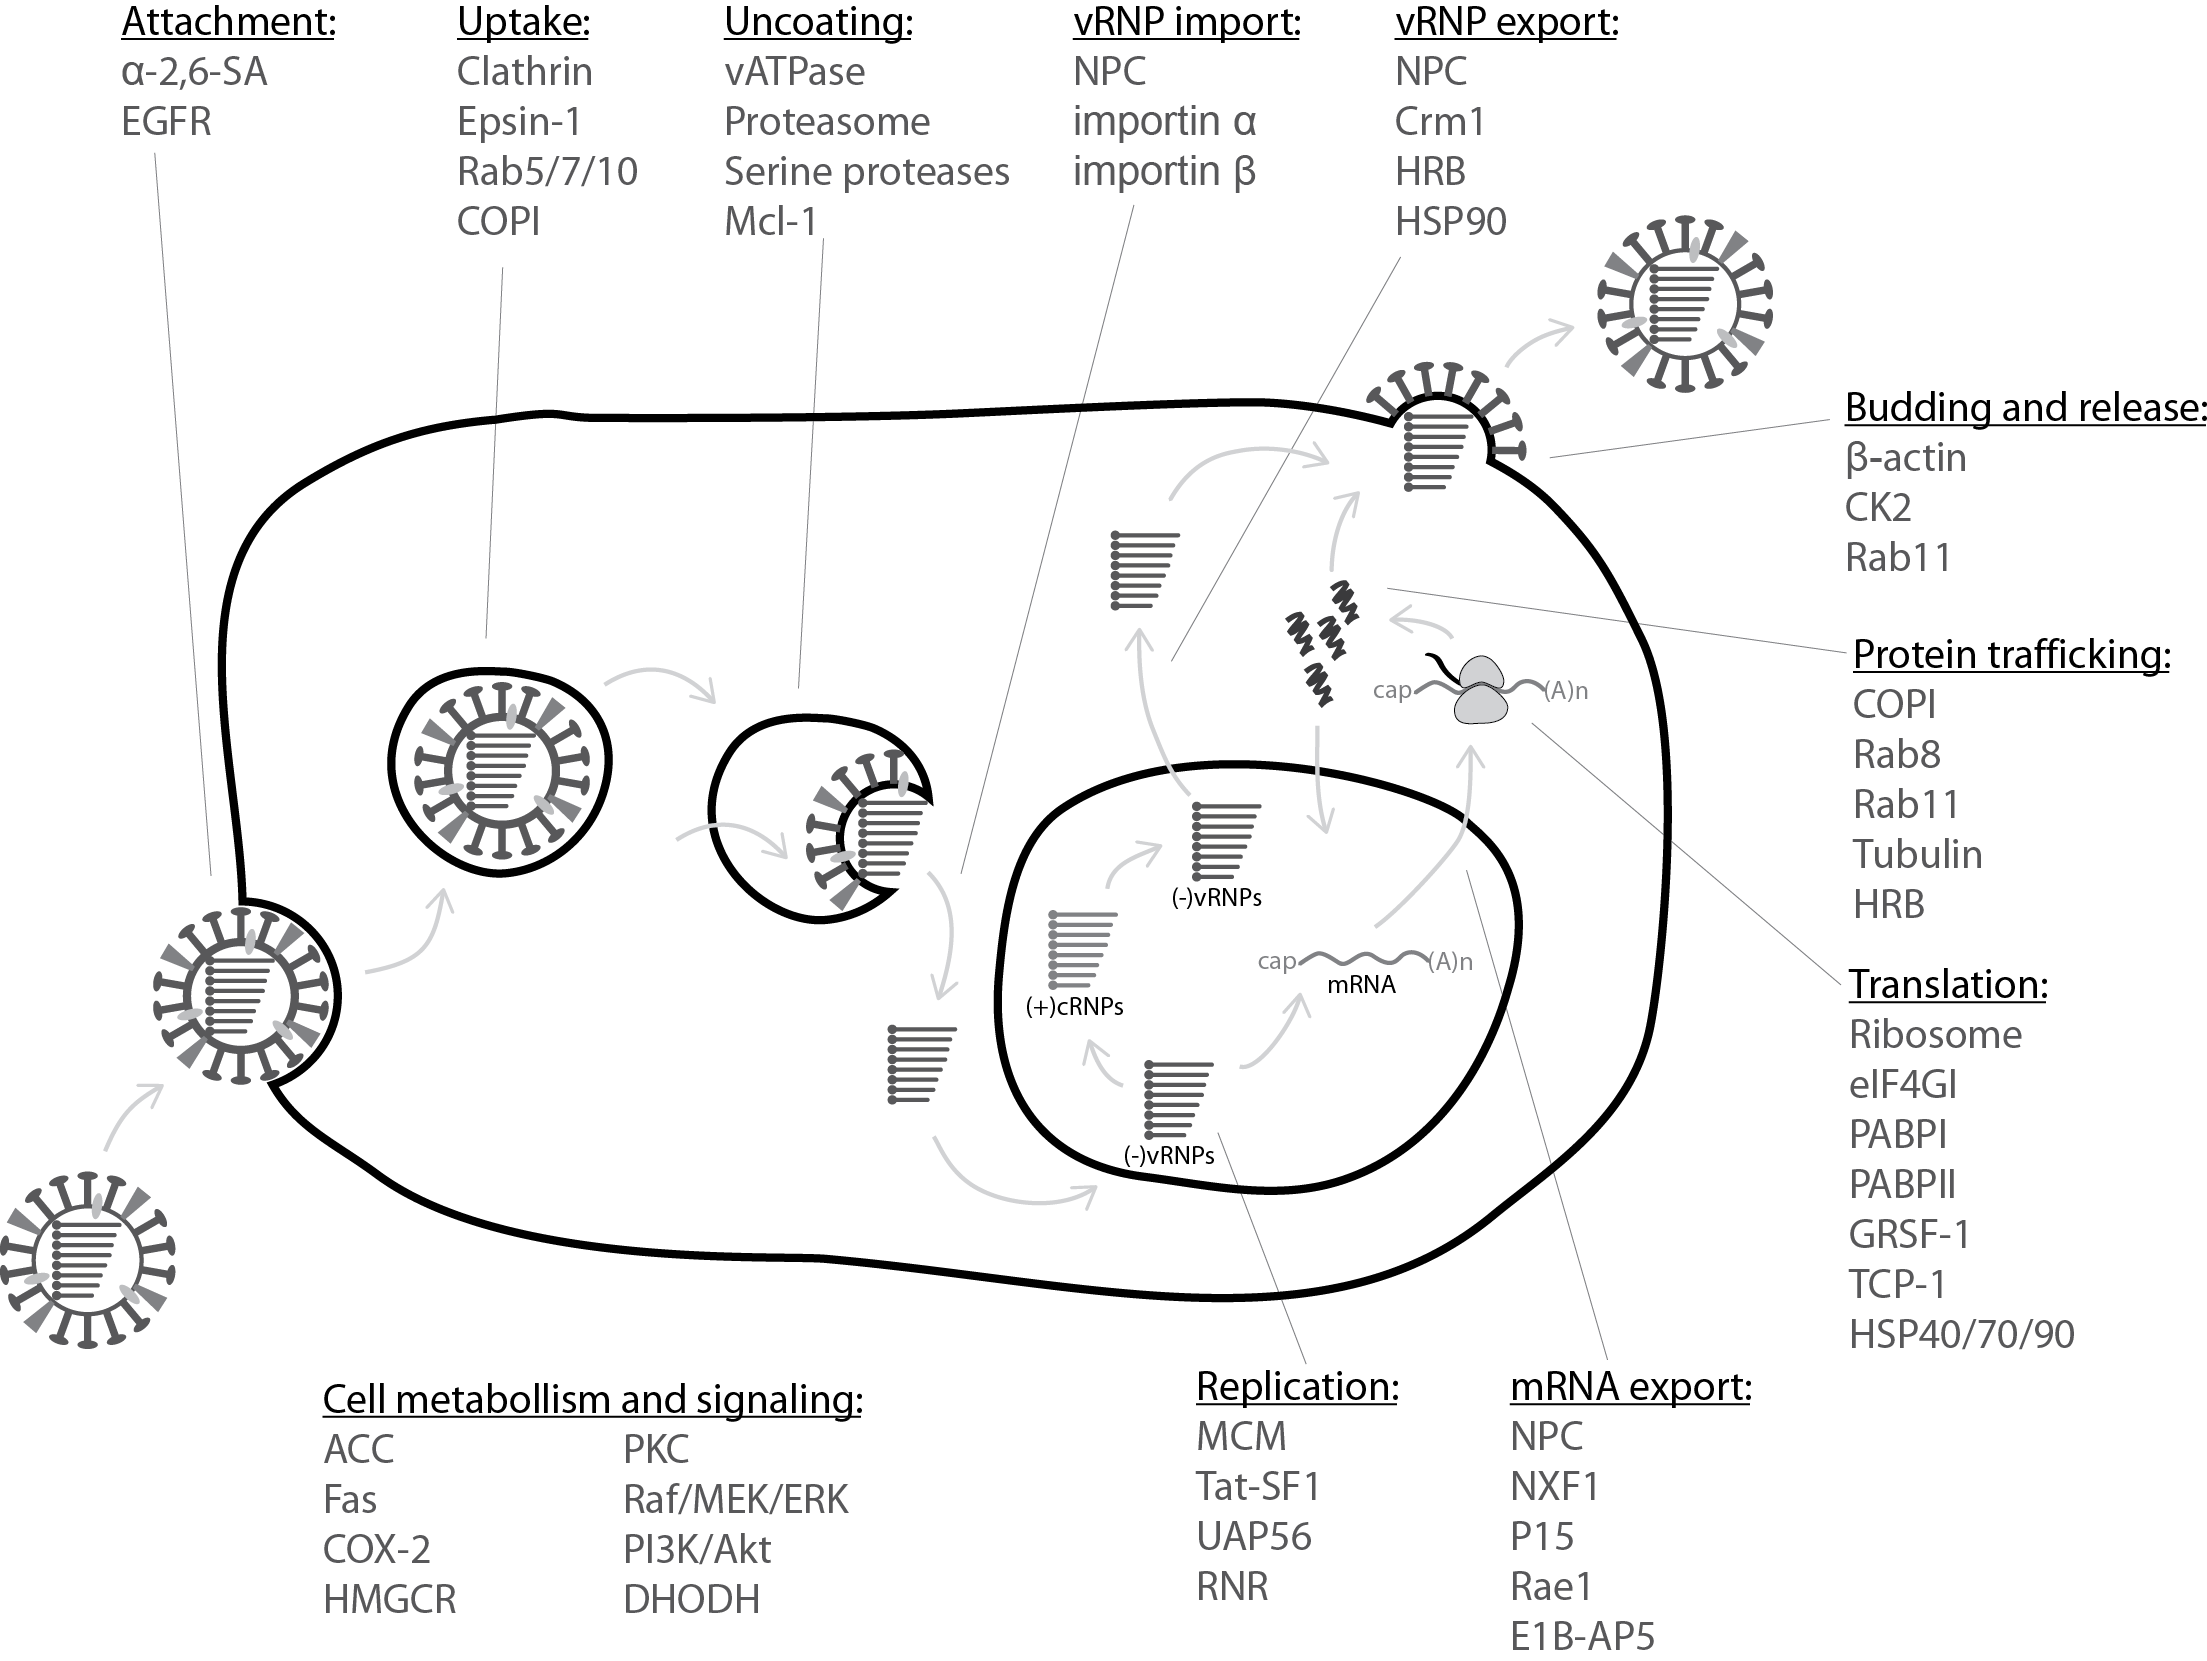
\includegraphics[width=\textwidth]{IAV_cycle.png}}
				\caption{Influenza A virus replication cycle and cellular factors involved in it. The abbreviated host factors are: $\alpha$-2,6-SA~--- $\alpha$-2,6-linked sialic acids; EGFR~--- epidermal growth factor receptor; COPI~--- coatomer 1 vesicular transport complex; vATPase, vacuolar H+-ATPase; Rab 5/7/8/10/11~--- small GTPases; Mcl-1~--- induced myeloid leukemia cell differentiation protein Mcl-1; NPC~--- nuclear pore complex; CRM1~--- exportin-1; HRB~--- HIV rev-binding protein; HSP40/70/90~--- heat shock protein 40, 70 or 90 kDa; CK2~--- casein kinase 2; Rab 8/11~--- small GTPases; eIF4GI~--- eukaryotic initiation factor 4 gamma 1; PABPI/II~--- polyadenylate-binding protein cytoplasmic isoforms I and II; GRSF1~--- G-rich sequence factor 1; TCP1, T-complex protein 1;  NXF1~--- nuclear mRNA export factor 1; P15~--- mRNA export factor; Rae1~--- mRNA export factor 1; E1B-AP5~--- heterogeneous nuclear ribonucleoprotein U-like protein 1; MCM~--- minichromosome maintenance complex IREF-1; Tat-SF1~--- Tat-specific factor 1; UAP56~--- helicase UAP56; RNR~--- ribonucleotide reductase; ACC~--- acetyl-CoA carboxylase; FAS~--- fatty acid synthase; COX-2~--- cyclooxygenase 2; HMGCR~--- 3-hydroxy-3-methylglutaryl-coenzyme A reductase; Raf/MEK/ERK~--- Ras/Raf/mitogen-activated protein kinase/extracellular signal-regulated kinase pathway; PI3K/Akt, phosphatidylinositol 3 kinase/RAC-alpha serine/threonine-protein kinase pathway; DHODH~--- dihydroorotate dehydrogenase.} \label{fig:cycle}
			\end{figure}	
	
	Effective synthesis of \glspl{vRNP} requires interaction of \gls{rdrp} with cellular minichromosome maintainance complex \parencite{Kawaguchi2007}, serine/threonine phosphatase 6 \parencite{York2014}. The export of \glspl{vRNP} is dependent on the interaction of \gls{M1}-\gls{vRNP} with the cellular nuclear export receptor Crm1, which presumably occurs via viral \gls{NEP} \parencite{Brunotte2014} and their further transport to the budding site requires interaction of viral \gls{NP} with cellular Rab11 GTPase \parencite{Eisfeld2011}. Finally, assembly of the virion at the budding site and bud formation requires functional actin microfilaments and cellular energy sources \parencite{Nayak2004}. 	The above mentioned interactions give just a few examples of a complex interactome that the virus establishes during infection: accession of host-pathogen interaction database  \parencite{Kumar2010} yielded published associations of viral proteins with over 400 host factors (\hyperref{http://www.agbase.msstate.edu/hpi/main.html}, accessed on 10.12.2014). 
	
	Influenza A replication triggers cellular antiviral responses and therefore its effectiveness is not limited to recruiting essential host factors but expands far beyond that. Establishment of tight control over cellular responses to infection is absolutely critical for successful viral replication in immune-competent system. 
	
			
	
	\subsection{Host responses to Influenza A infection}
	
	The hosts of influenza A virus have evolved defensive mechanisms to protect themselves from infections by preventing viral entry into the cell, reducing the viral burden or diminishing the negative consequences of infection. These mechanisms are realized through three lines of host defense: the intrinsic physicochemical barriers, the innate immunity and the adaptive immunity.
	
	In mammals influenza A is transmitted mainly through aerosols and droplets and enters the host through the respiratory tract \parencite{Brankston2007}. The first line of antiviral defense in the respiratory tract is represented by the airway mucus. It consists mainly of glycoproteins and antimicrobial and antiviral substances and is an essential barrier for virus infection \parencite{Thornton2008, Nicholas2006}. The viruses that penetrate the airway mucus barrier initiate infections of the respiratory tract epithelial cells and can also spread to immune cells of the respiratory tract, mainly macrophages and \glspl{DC} \parencite{Perrone2008, Bender1998}. Infection of susceptible cells with influenza A is rapidly detected by specific sensors which trigger induction of innate immune responses. Such responses include activation of antiviral gene expression and production of effector molecules that regulate innate immune signaling in autocrine and paracrine manner \parencite{Iwasaki2014}. The efficiency of these processes is critical for restriction of viral burden and for informing the adaptive immunity~--- the third line of host defense essential for clearance of the infection site and generation of immune memory \parencite{Iwasaki2010}. 
	
	Although cellular responses involve a complex network of events that are hard to tackle, in recent years substantial progress has been made towards our understanding of critical processes that regulate virus detection, antiviral signaling and activation of immune-related genes.
	
		\subsubsection{Detection of the virus}
		
		Eukaryotic cells evolved a way to distinguish between ``self'' and ``non-self'' via expression of specific detection molecules called \glspl{PRR} \parencite{Janeway2002}. These \glspl{PRR} recognize specific molecular signatures produced by invading microorganisms that are called  \glspl{PAMP} and initiate downstream signaling events to activate innate immune responses \parencite{Janeway1989}.The current paradigm of innate immunity to influenza A virus assumes during replication the virus produces three types of  \glspl{PAMP}. These \glspl{PAMP} are single- and double-stranded viral RNA and 5' triphosphates generated during viral genome synthesis by \gls{rdrp} \parencite{Guillot2005, Hornung2006, Kato2006, Lund2004}. They are recognized in the endosome or in the cytoplasm by three major classes of cellular \glspl{PRR}: \glspl{NLR}, \glspl{TLR}, and \glspl{RLR} \parencite{Iwasaki2014}. 
		
		Viral recognition in the endosome relies on three different \gls{TLR} class members: \gls{TLR}3 which recognizes dsRNA, \gls{TLR}7 and \gls{TLR}8 which recognize ssRNA \parencite{Iwasaki2014}. 
		
		\gls{TLR}3 is constitutively expressed in pulmonary and airway epithelial  cells and in \glspl{DC} \parencite{Guillot2005, Schulz2005, Ioannidis2013}. It has been initially shown to recognize dsRNA and induce \gls{IFN} production in response to it \parencite{Alexopoulou2001, Guillot2005}. \gls{TLR}3 signaling is activated in response to replicating influenza A virus \parencite{Guillot2005}. 	\gls{TLR}7 is expressed by airway epithelial cells and \gls{DC}s and plasmocytoid \gls{DC}s \parencite{Ioannidis2013, Lund2004}. \gls{TLR}7 can be activated by \gls{ssRNA} and is proposed to recognize genomic vRNA of influenza A virus in the endosome \parencite{Diebold2004}. Unlike other \glspl{TLR}, \gls{TLR}8 has been so far only found in macrophages and monocytes where it is activated in response to \gls{ssRNA} and 5' triphosphates \parencite{Ablasser2009}. Its signaling is activated upon influenza A infection and leads to production of \gls{IL}-12, however the distinct role of \gls{TLR}8 in regulation of innate immunity is yet to be determined \parencite{Lee2013a}.
		
		%However, the mechanism for its activation is unclear, as influenza A viruses do not produce detectable amounts of dsRNA during their replication due to activity of cellular RNA helicase UAP56 \parencite{Wisskirchen2011}. In \glspl{DC}, \gls{TLR}3 signaling is activated upon phagocytosis of infected material, suggesting their localization of \gls{TLR}3 in the endosome \parencite{Schulz2005}. 
		
		The listed \gls{TLR}s are expressed in endosomal compartments of the cells, except \gls{TLR}3, which was also found in the outer membrane \parencite{Schulz2005, Ablasser2009, Diebold2004}. The proposed mechanisms for their activation in response to influenza A are, however, unclear for three reasons: (i) influenza A does not produce detectable amounts of dsRNA during its replication due to activity of cellular RNA helicase UAP56 \parencite{Wisskirchen2011}; (ii) paired 5' and 3' ends of vRNA are bound to viral \gls{rdrp}, which can hinder 5' triphosphates from their recognition by \glspl{TLR} \parencite{Arranz2012}; and (iii) of all \glspl{TLR} that recognize influenza A virus, only \gls{TLR}7 seems to be critical for viral recognition \parencite{Lund2004}. However, it is not clear whether it recognized any specific structures or sequences within RNA trigger \gls{TLR}7 activation, as  was shown readily recognizes both ``self'' and ``non-self'' RNA \parencite{Diebold2004}.
		
		%The plausible explanation of influenza A \glspl{PAMP} detection by \glspl{TLR} might be that 
		
		%However, as in the genomic vRNA is packaged in \gls{vRNP} structures and encapsidated in the virion, the details of its recognition by \gls{TLR}3 are unclear \parencite{Diebold2004}. Neither is it known whether any specific structures on vRNA are sequired for \gls{TLR}7 activation, as it seems to be both sequence- and structure unspecific, as it readily recognizes both ``self'' and ``non-self'' RNA and it is proposed that its endosomal localization if the way to avoid binding ``self'' RNA and secure binding of vRNA \parencite{Diebold2004}. I.
				
		TLR7 and TLR8 interact with their common adapter MyD88 \parencite{Medzhitov1998}. MyD88 recruits IRAK family kinases which mediate phosphorylation and nuclear translocation of \gls{IRF}3 and \gls{IRF}7~--- transcription factors that induce \textit{\gls{IFN}} gene expression \parencite{Burns2003, Honda2005a}. In addition, MyD88 activates \glspl{MAPK} signaling and transcription factor \gls{AP1}, that controls expression of proinflammatory genes \parencite{Kawai2007}. TLR3 induces its signaling via interaction with \gls{TRIF} and its downstream pathways bifurcate \parencite{Guillot2005, Kumar2009}. One induces type I \gls{IFN} production via TBK1 and \gls{IKK} kinases and \gls{IRF}3, \gls{IRF}7. Another stimulates production of proinflammatory cytokines via \gls{IKK} and \gls{NFkB} or via \gls{MAPK} signaling and transcription factor \gls{AP1} \parencite{Guillot2005, Vercammen2008}.  
		 
		Viral recognition in the cytoplasm relies on \glspl{RLR} and \glspl{NLR}.
		\glspl{RLR} is a group of helicases that named after its representative \gls{RIG-I}. \glspl{RLR} are constitutively present in low amounts in multiple cell types, but their most prominent location is airway epithelium \parencite{Bogefors2011} where they play an essential role in detection of airborne pathogens. \gls{RLR} group consists of three proteins: \gls{RIG-I}, \gls{MDA5} and \gls{LGP2} \parencite{Kang2004, Yoneyama2004, Yoneyama2005}. They are structurally similar and contain RNA-binding \gls{CTD} and a DExD/H box helicase domain \parencite{Cui2008, Takahasi2009}. \gls{RIG-I} and \gls{MDA5} also contain two consecutive N-terminal \glspl{CARD} that mediate signaling \parencite{Yoneyama2004, Kang2004}. All \glspl{RLR} recognize dsRNA, and \gls{RIG-I} can also recognize ssRNA with 5' triphosphates \parencite{Cui2008}. 
		
		In the cytoplasm \gls{RIG-I} is normally present in an inactive autorepressed state in which its \glspl{CARD} are sequestered by the helical domain, preventing non-specific induction of \gls{RIG-I} downstream signaling \parencite{Kowalinski2011}. Upon sensing its ligands by \gls{CTD}, \gls{RIG-I} undergoes conformational rearrangement which liberates its \glspl{CARD} for downstream signaling \parencite{Kowalinski2011}. Activation of \gls{RIG-I} is  dependent on its ubiquitination by E3 ubiquitin ligases TRIM25 and RIPLET or on binding to free polyubiquitin chains generated by TRIM25. Both TRIM25 and RIPLET are required for \gls{RIG-I} signaling \textit{in vitro} and \textit{in vivo} \parencite{Gack2007, Oshiumi2010, Zeng2010}. The modified \gls{RIG-I} oligomerizes \parencite{Patel2013}, and undergoes additional conformational rearrangements that enable interaction with its adapter \gls{MAVS} \parencite{Kawai2005, Seth2005}. For this, \gls{RIG-I} is targeted to mitochondria in a ``translocon'' complex containing TRIM25 and mitochondrial targeting chaperone 14-3-3$\epsilon$ \parencite{Liu2012}. Upon binding \gls{RIG-I}, \gls{MAVS} oligomerizes and forms a scaffold for a multi-kinase signaling complex which includes \gls{JNK}, \gls{TBK1} and \gls{IKK}$\epsilon$ complex, and \gls{IKK}$\alpha$/$\beta$/$\gamma$ complex \parencite{McWhirter2005}. These kinases eventually activate transcription factors \gls{IRF}3, \gls{AP1} and \gls{NFkB} which regulate type I \gls{IFN} genes \parencite{McWhirter2005}. A simplified scheme of \glspl{TLR} and by \gls{RIG-I} signaling is shown on Figure \ref{fig:detection}.
		
		The only \gls{NLR} that detects influenza A is \gls{NLRP3} found in lung and bronchial epithelial cells, monocytes, macrophages and \gls{DC}s \parencite{Guarda2011, Kim2014}. It is constitutively present in an inactive form in the cell cytoplasm. During influenza A infection \gls{NLRP3} is activated by sensing viral \gls{ssRNA} or proton flux mediated by viral \gls{M2} in trans Golgi network \parencite{Thomas2009, Ichinohe2010, Allen2009}. Virus-mediated activation and oligomerization of \gls{NLRP3} leads to formation of inflammasome~--- a multiprotein complex that includes \gls{NLRP3}, \gls{ASC} and pro-caspase 1 \parencite{Tschopp2010}. Inflammasome is required for proteolytic self-activation of pro-caspase 1, which afterwards cleaves and activates IL1$\beta$ and IL18 precursors.
	
		Whereas \gls{RIG-I} activation results in induction of antiviral responses by \gls{IFN}s and \gls{ISG}s, signaling by \gls{NLRP3} and \glspl{TLR} can also induce pro-inflammatory responses (see section 1.5.3. for more details) \parencite{LeGoffic2007, Allen2009, Kawai2007}. 
		
		\begin{figure}[h]
			\centering
			\fbox{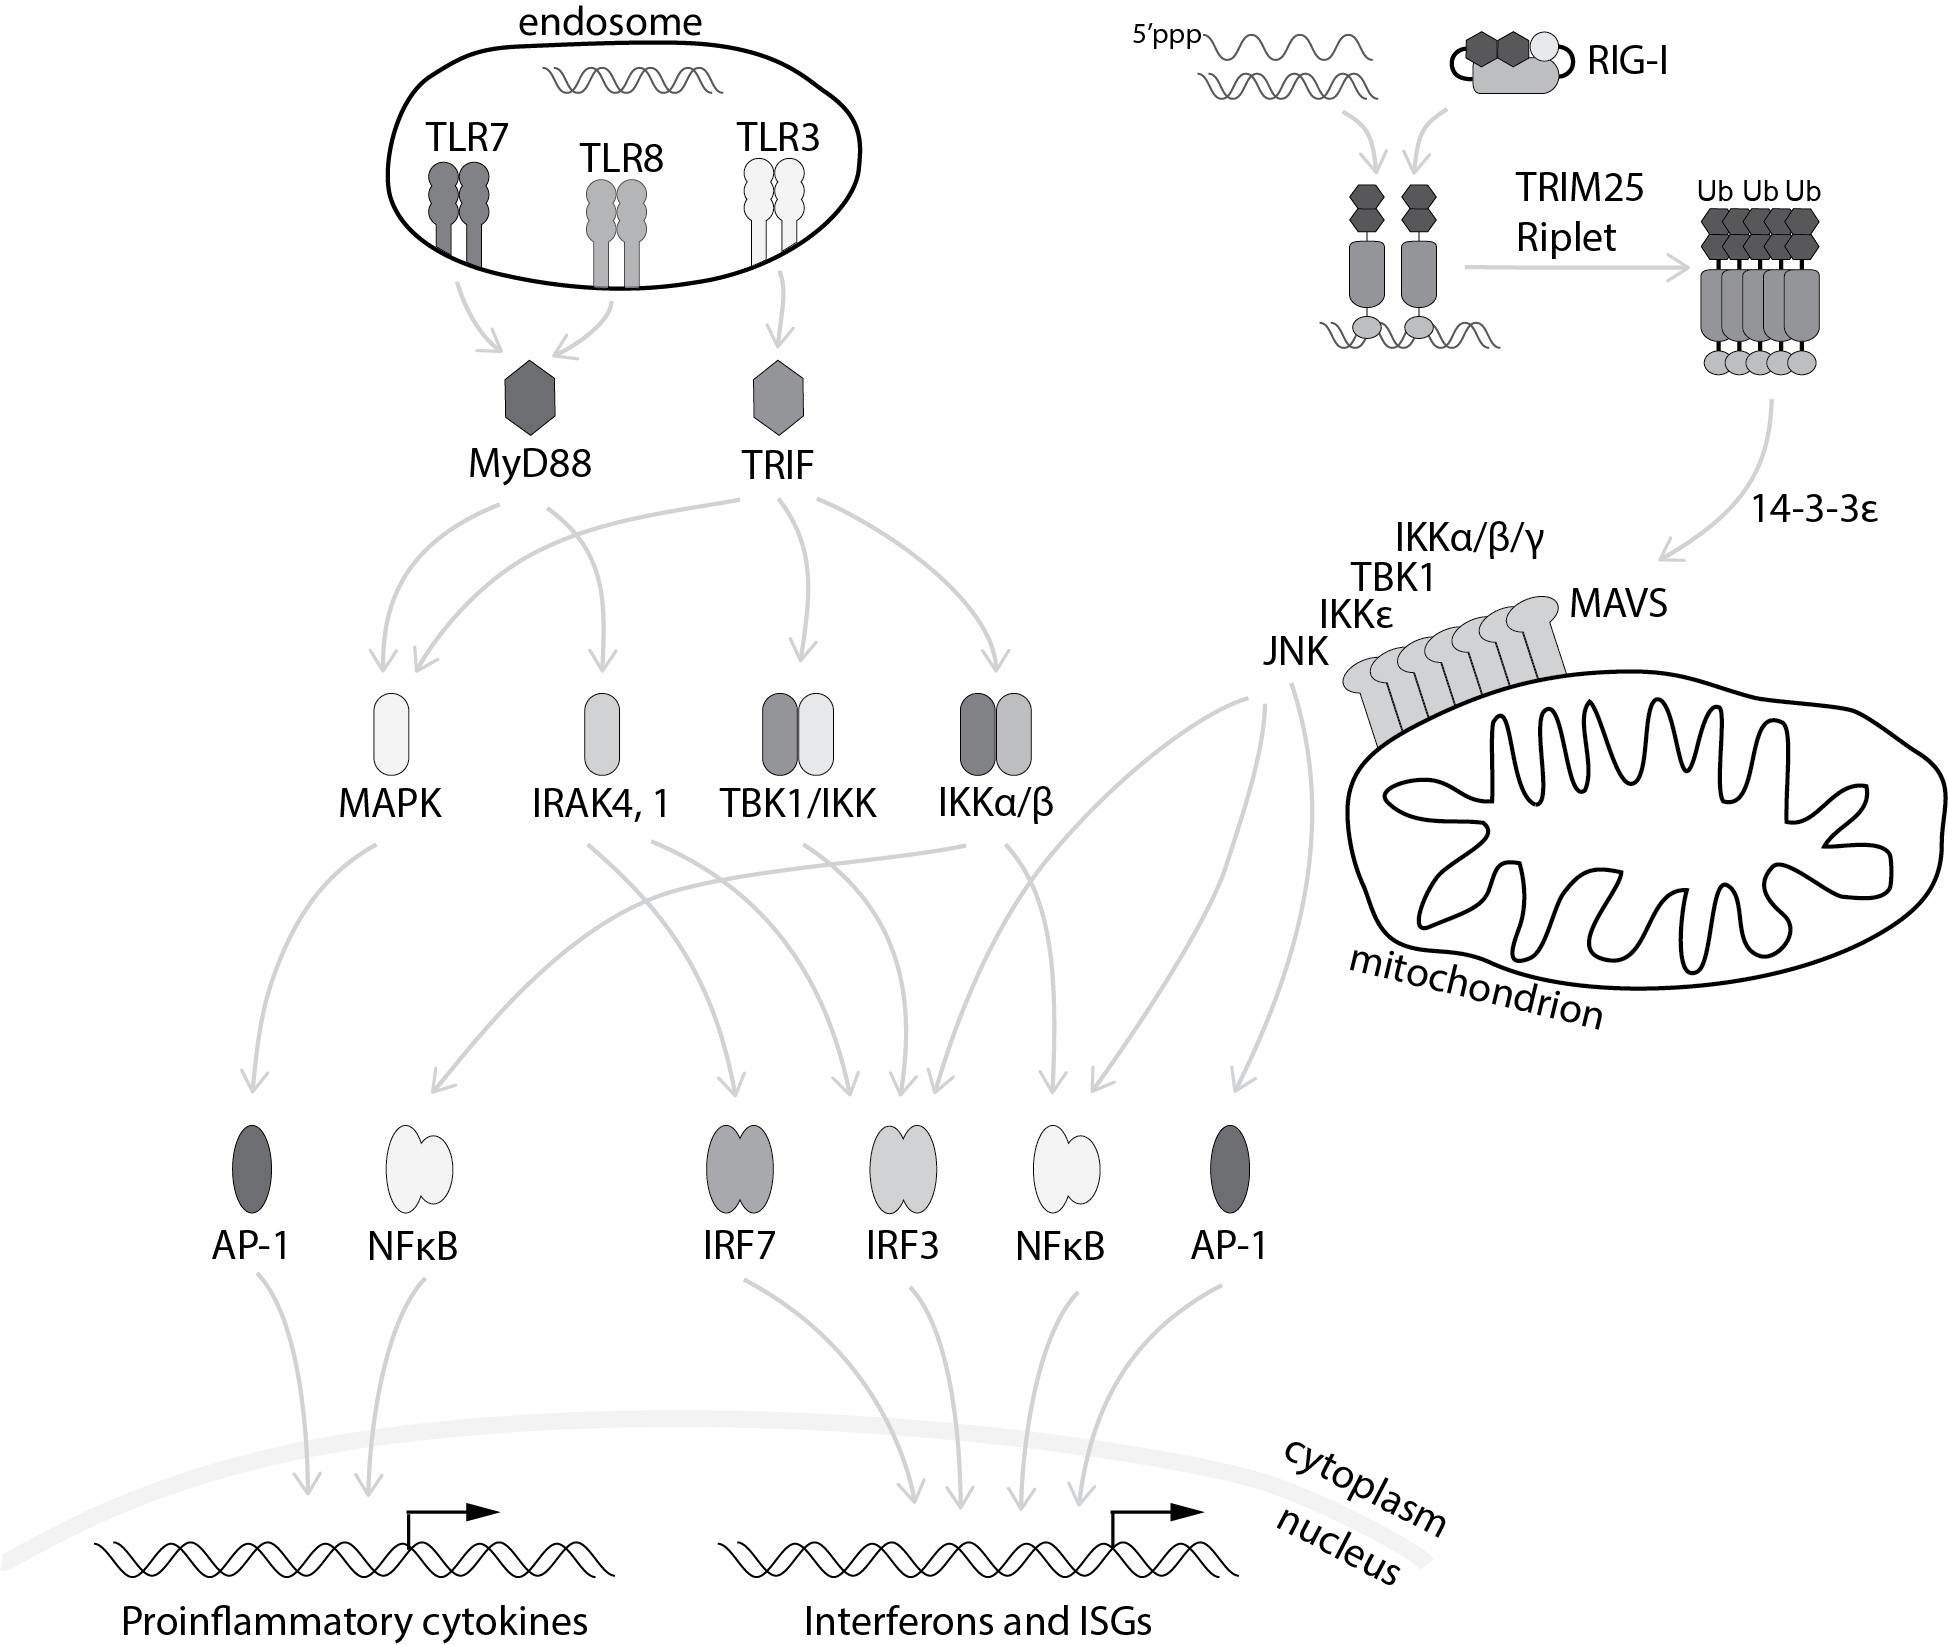
\includegraphics[width=\textwidth]{virus_detection.png}}
			\caption{\glspl{TLR} and \gls{RIG-I} activation and downstream signaling.} \label{fig:detection}
		\end{figure}	
		%Detection of the virus by TLR3 activates so-called ``proinflammatory'' responses\parencite{LeGoffic2007} to IAV that result in production of ILs 6,8, 12p40/p70, RANTES and are required for establishment of inflammation. proliferation of CD8+ CTLs. Detection of the virus bt RIG-I results in ``antiviral'' signaling \parencite{LeGoffic2007} whereby production of type I IFNs activates expression of interferon-stimulated genes, which products modulate cellular processes to restrict viral replication.
		
		%The activation of \glspl{TLR} controls type I interferons and proinflammatory cytokines \parencite{Kawai2007}. 
		
		\subsubsection{Antiviral responses by interferons and interferon-stimulated genes}
		
		Followng detection of viral \gls{PAMP}s and establishment of \gls{PRR} signaling, the infected cells produce and secrete small regulatory proteins known as interferons \parencite{Fensterl2009}. Interferons are subdivided into three types (I--III) based on their respective receptors  \parencite{Branca1981, Sheppard2003}. Autocrine and paracrine types I and III \gls{IFN} signaling activates \gls{ISG}s and antiviral responses \parencite{Kotenko2003, Garcia-Sastre2006}, reinforces \gls{PRR} production \parencite{Pothlichet2013}, and regulates adaptive responses via enhancement of antigen presentation to CD4\textsuperscript{+} and CD8\textsuperscript{+} T-cells \parencite{Zietara2009}.
	
		Both type I and III \glspl{IFN} are secreted by nearly all cell types, although the majority is secreted by \glspl{DC} \parencite{Siegal1999, Odendall2014}. Type I \glspl{IFN} include \gls{IFN}$\alpha$ and \gls{IFN}$\beta$ and utilize dimeric receptor IFNAR1/IFNAR2 on cell surface \parencite{Mogensen1999}. Type III \glspl{IFN} are \gls{IFN}$\lambda$1, \gls{IFN}$\lambda$2, \gls{IFN}$\lambda$3 (also called \gls{IL}29, \gls{IL}28A and \gls{IL}28B, respectively), and \gls{IFN}$\lambda$4. They bind to their heterodimeric receptor IL10R2/IFNLR1 \parencite{Kotenko2003, Sheppard2003}. Both type I and III \gls{IFN} receptors activate signaling through the \gls{JAK} / \gls{STAT} pathway. Binding of \gls{IFN} to its receptor triggers a series of phosphorylation events in which receptor-bound \gls{JAK} phosphorylates itself, the \gls{IFN} receptor and receptor-associated proteins \gls{STAT}1 and \gls{STAT}2 \parencite{VanBoxel-Dezaire2006}. Phosphorylation of \gls{STAT}1 and \gls{STAT}2 triggers their heterodimerization and formation of regulatory complex with \gls{IRF}9 \parencite{Fu1990}. This complex is translocated to the nucleus where it transcriptionally activates \glspl{ISG} \parencite{Levy1988}. A schematic illustration of type \gls{IFN} induction is present of Figure \ref{fig:IFN}.
		
		\glspl{ISG} are diverse group of genes that control multiple cellular processes: they enhance virus sensing by \gls{PRR}s, can target pathways essential for viral replication, upregulate cytokine and chemokine production, control \gls{IFN} response via positive and negative feedback loops. The best-described \gls{ISG}s with antiviral action include \gls{MxA}, \gls{IFITM3}, \gls{CH25H}, \gls{ISG15}, \gls{PKR}, and \gls{OAS}. 
		
		\gls{CH25H} and \gls{IFITM3} exert their antiviral activity during virus entry. \gls{CH25H} converts cholesterol in 25-hydroxycholesterol which   protects against influenza \parencite{Blanc2013}. The proposed mechanism for viral inhibition by \gls{CH25H} is that increased concentrations of 25-hydroxycholesterol in cellular membranes alter their properties and inhibit viral fusion in late endosomes \parencite{Liu2013}. \gls{IFITM3} is localized in late endosomes where it is also thought to alter properties of endosomal membrane and prevent virus fusion \parencite{Li2013, Desai2014}. 
				
		Human \gls{MxA} gene product is a dynamin-like \gls{GTPase} \parencite{Nakayama1992}. It is localized in the cytoplasm of infected cells where it self-assembles into ring-like ordered structures \parencite{Gao2010}. Although the detailed mechanism of its antiviral activity is yet do be established, \gls{MxA} oligomers presumably recognize and bind \gls{vRNP}s in the cytoplasm, preventing their nuclear import and thus attenuate influenza A replication \parencite{Haller2010}.
		
		\gls{PKR} and \gls{OAS} act at later stages of viral replication cycle. \gls{PKR} is a multifunctional serine/threonine kinase that has a critical role in host antiviral responses \parencite{Garcia2006a}. It is constitutively present cytoplasm at low abundancy, and its expression is trancsriptionally induced by type I and III \gls{IFN}s \parencite{Meurs1990}. \gls{PKR} is activated via its interaction with dsRNA or \gls{PACT} \parencite{Li2006a}. It phosphorylates and inactivates translation initiation factor \gls{eIF2a} \parencite{Levin1978}. \gls{eIF2a} is indispensable for initiation of cap- and often of \gls{IRES}-driven translation, and thus activation of \gls{PKR} in response to virus infection shuts down protein synthesis \parencite{Kimball1999}. In addition to controlling protein synthesis in infected cells, \gls{PKR} can also detect dsRNA, mediate \gls{IFN}$\gamma$-induced \gls{NFkB} activation \parencite{Deb2001}, modulate \gls{STAT}1 signaling \parencite{Wong1997}, induce \gls{JNK} and \gls{MAPK} signaling in response to viral infection \parencite{Chu1999}, induce apoptosis and autophagy following the shut down of protein synthesis \parencite{Gil2000, Talloczy2002}. \gls{PKR} mediates death of infected cells unless the virus counteracts its action \parencite{Takizawa1996, Hatada1999}. As no cytoplasmic dsRNA is  detectable during influenza A replication \parencite{Wisskirchen2011}, \gls{PKR} activation during infection is likely mediated by \gls{TLR} signaling \parencite{Jiang2003} or by binding to its protein activator \parencite{Garcia2006a}.
		
		\gls{OAS} and \gls{RNAseL} act together in the antiviral RNA decay pathway. Both enzymes are upregulated by \gls{IFN}, but they are also present constitutively in cell cytoplasm \parencite{Sadler2008}. Like \gls{PKR}, \gls{OAS} can be activated by binding to dsRNA \parencite{Castelli1998}. Upon its activation, \gls{OAS} synthesizes 2'-5'-linked adenosine triphosphate oligomers, which, in turn, act as inducers of latent \gls{RNAseL} \parencite{Rebouillat1999}. Activated \gls{RNAseL} catalyzes endonucleolytic degradation of cellular and viral ssRNAs and mRNAs thus contributing to host antiviral responses \parencite{Dyer2006}. In addition to viral RNA elimination, \gls{RNAseL} reinforces virus detection by \gls{TLR}s and \gls{RIG-I} and \gls{IFN} response, and regulates apoptosis in infected cells \parencite{Liang2006}. Replication of influenza A virus unable to inhibit \gls{OAS}/\gls{RNAseL} pathway is attenuated \parencite{Min2006}.
		
		Some \gls{ISG}s are also implicated in interferon responses control via negative feedback loops \parencite{Schneider2014}. SOCS proteins inhibit JAK/STAT signaling \parencite{Hong2013} and USP18 binds to inhibits IFNAR2  \parencite{Ritchie2004}.
		
		\begin{figure} %[h]
			\centering
			\fbox{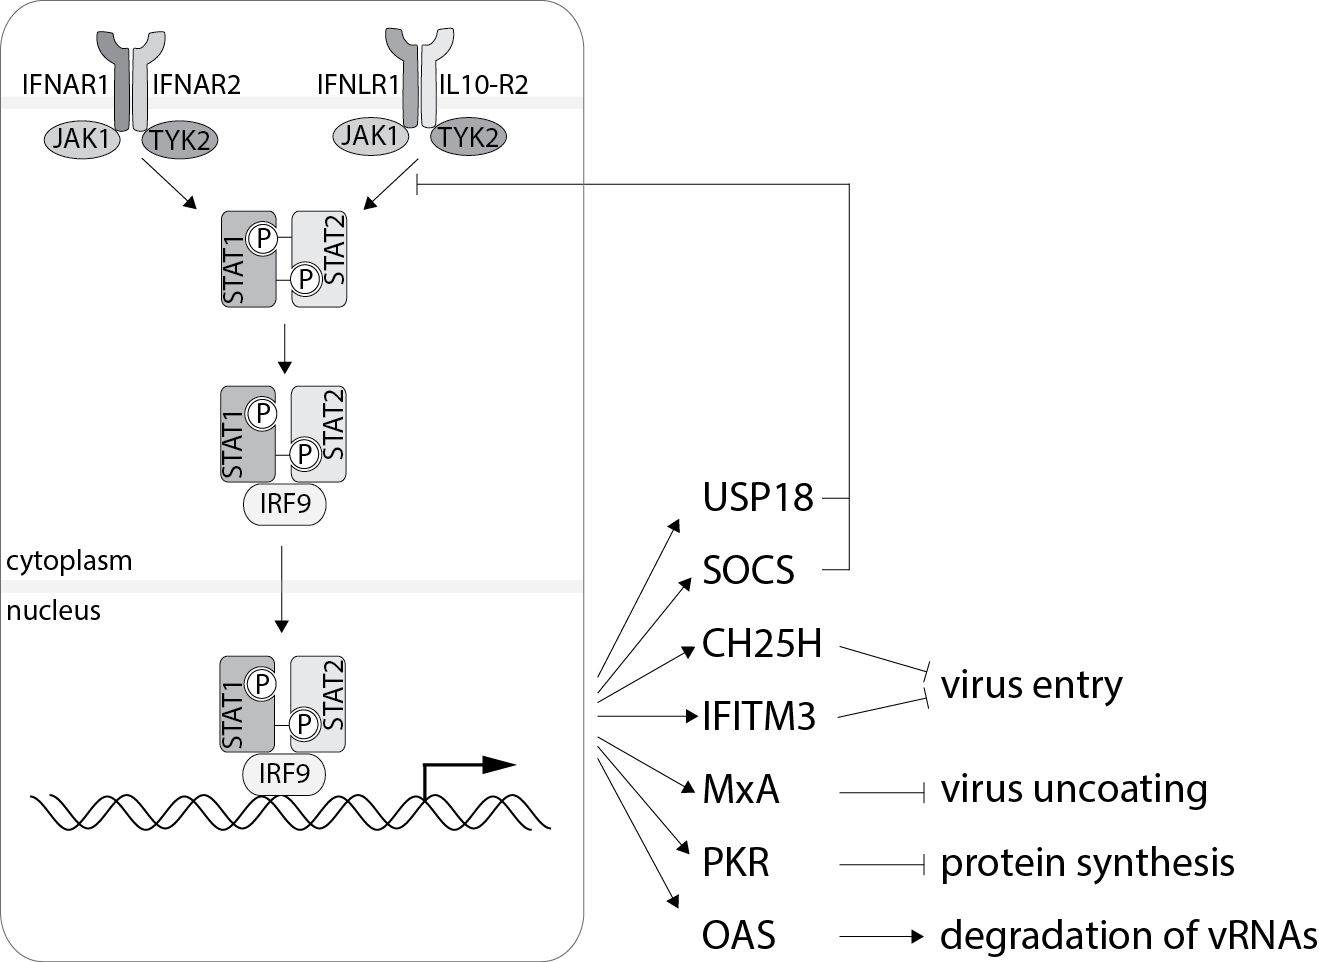
\includegraphics[width=\textwidth]{IFN.png}}
			\caption{A schematic representation of Type I and III \gls{IFN} responses induction.} \label{fig:IFN}
		\end{figure}
		
		
		
		\subsubsection{Pro-inflammatory responses}
		
		Pro-inflammatory responses induced by \gls{TLR} and \gls{NLRP3} signaling activate production of chemokines including IL1-$\beta$, IL6, IL8, IL18, RANTES, MCP-1, MCP-3 and MIP-3$\alpha$ \parencite{Julkunen2000, LeGoffic2007}. Unlike type I \glspl{IFN}, proinflammatory cytokines may not induce direct antiviral resistance, but are required for antigen presentation, establishment of inflammation, and recruitment of leukocytes to the site of infection and proliferation of CD8\textsuperscript{+} \glspl{CTL} \parencite{VanDerSluijs2005, Schulz2005, LeGoffic2006}. Consequently, they do not inhibit viral replication, but are essential for host resistance to infection \parencite{Pang2013}. In addition, the correct onset of proinflammatory responses regulates adaptive immunity to influenza A infection \parencite{Trinchieri2003, Ichinohe2009}. However, robust induction of proinflammatory response to some influenza A subtypes, e.g. H5N1, can be detrimental to the host and lead to severe immunopathology, thereby increasing viral pathogenicity \parencite{LaGruta2007}.	
			
		\subsubsection{Apoptosis}
		
		In addition to activating antiviral and pro-inflammatory responses, influenza A was shown to induce apoptosis in infected cells \parencite{Fesq1994, Hinshaw1994, Mori1995, Brydon2005}. The central role in apoptotic response belongs to cysteinyl proteases (caspases) which proteolytically inactivate numerous cellular proteins leading to cell death \parencite{Cohen1997, Thornberry1998}	
		
		A variety of cellular signaling pathways, including \gls{MAPK}, \gls{NFkB}, \gls{PKR} and \gls{PI3K}/Akt, are implicated in apoptosis regulation during infection \parencite{Gil2000, Xing2010, Lu2010}. Activation of apoptosis can play a role in host defense mechanism, by facilitating premature cell death and also by triggering production of pro-inflammatory cytokines \parencite{Julkunen2000}. It also contributes to viral clearance in cell culture and \textit{in vivo} being essential for CD8\textsuperscript{+}-mediated killing of infected cells \parencite{Ishikawa2005, Brincks2008}. On the other hand, onset of apoptic responses can be beneficial for the virus and influenza A propagation is attenuated in the presence of caspase inhibitors due to retention of \glspl{vRNP} in the nucleus \parencite{Wurzer2003}. Due to this twofold role of apoptosis in influenza A infection, it is tightly controlled by both cellular and viral factors.
			
		%ISG15 It is made up of two ubiquitin-like domains, in which the C-terminal LRLRGG motif is responsible for its conjugating (ISGylation) onto target proteins (23, 24). Formation of this isopeptide bond is catalyzed consecutively by a series of inducible enzymes:E1activating enzymeUbe1L(25),E2 conjugating enzyme UbcH8 (26, 27), E3 ligase Herc5 or EFP (28– 30), and deconjugating enzyme UBP43 (31). Unlike ubiquitination, ISGylation typically does not promote degradation of the target proteins. A couple of proteomics studies have identified .100 cellular proteins as potential targets of ISGylation (32–35). These proteins cover a wide spectrum of biological processes, including transcriptional regulation, signal transduction, inflammation, and control of cell growth. Notably, ISG15 and its conjugation system (E1, E2, and E3) were overexpressed in these proteomics studies, which made the observations possibly artificia
		
		
	\subsection{Viral means to counteract antiviral responses}
	
	Successful counteraction of antiviral responses is critical for influenza A replication and several viral proteins support replication cycle progression in the context of immune response. For instance, \gls{NA} cleaves sialic acids in host mucus to facilitate viral penetration \parencite{Cohen2013}, \gls{PB1}-F2 inactivates \gls{RIG-I}/\gls{MAVS} and \gls{NFkB} signaling \parencite{Varga2011a, Dudek2011, Reis2013}, and \gls{NP} mediates resistance to \gls{MxA} \parencite{Dittmann2008}. Both \gls{PB1}-F2 and \gls{M2} can contribute to regulation of apoptosis during infection \parencite{Herold2012}. However the critical role in inhibition of antiviral responses and regulation of virus-host interactions is assigned to \gls{NS1} \parencite{Garcia-Sastre1998}. Indeed, viruses lacking functional \gls{NS1} are severely attenuated, especially in immune-competent systems, and can only replicate in the absence of \gls{STAT}1 or \gls{PKR} \parencite{Garcia-Sastre1998, Egorov1998, Donelan2003, Falcon2004}. Due to its critical role in viral replication \gls{NS1} has been extensively studied and its roles in regulation of virus-host interactions stretch beyond regulation of \gls{IFN} responses and include regulation of vRNA synthesis, enhancement of viral protein synthesis, regulation of virion assembly, modulation of cellular signaling, apoptosis inhibition, contribution to host range definition and pathogenesis. 
		
	\subsection{NS1 protein}
		
		\gls{NS1} is a non-structural protein, but it is expressed in high quantities in infected cells \parencite{Ritchey1976}. Initial studies indicated that \gls{NS1} is essential for viral replication \parencite{Koennecke1981} and further investigations proved that it is a versatile viral protein which is a key regulator of influenza A virus-host interactions \parencite{Ayllon2015}.
		
		\subsubsection{NS1 synthesis and localization}
		
		The mRNA of \gls{NS1} is generated by colinear transcription of the 8\textsuperscript{th} genomic segment (NS). About 10 \% of NS transcripts are spliced and generate the mRNA of another viral protein, \gls{NEP} \parencite{Lamb1980}, which shares the first 10 amino acids with \gls{NS1} \parencite{Inglis1979, Lamb1979, Lamb1980}. As \gls{NS1} is not found in virions, it appears in infected cells only after viral transcripts have been generated and translated. Although intracellular localization of \gls{NS1} may vary depending on its abundance, the virus isolate, cell type and polarity, and time post infection, the majority \gls{NS1} is localized in cellular nucleus, but a fraction of it is also present in the cytoplasm\parencite{Melen2007, Melen2012, Newby2007, Li1998, Greenspan1988}. 
		
		Generally, proteins of up to ~60 kDa can be imported in the nucleus by passive diffusion \parencite{Macara2001, Wang2007} which does not require specific \gls{NLS}. \gls{NS1} is a relatively small protein and its molecular mass is only 26 kDa \parencite{Ward1994}, however, its nuclear import occurs in an active way. Depending on the virus subtype, \gls{NS1} can contain one or two \glspl{NLS} which mediate interaction with cellular importin-$\alpha$ \parencite{Melen2007}, thus securing rapid nuclear import of \gls{NS1} \parencite{Privalsky1981}. The monopartite \gls{NLS}1 is located close to the protein N-terminus, involves aa R35, R38 and K41, and is conserved across most influenza A isolates. The bipartite C-terminal NLS2 is present in a subset of viral strains expressing extended 237 \gls{aa} \gls{NS1}. It is located around \gls{aa} 219--237 and also serves as a \gls{NoLS} \parencite{Melen2007, Melen2012}. Cytoplasmic localization of \gls{NS1} seems to depend on \gls{NES} which lies within residues 138--147 \parencite{Li1998}. This \gls{NES}, however, is masked by adjacent residues 148--161 and its activation requires ``unmasking'' which presumably occurs via the conformational change upon interaction of \gls{NS1} with and unidentified protein partner(s). 
		
		\subsubsection{Post-translational modifications of NS1}
		
		%In infected cells a significant fraction of \gls{NS1} can be post-translationally modified. These modifications include phosphorylation, linkage of \gls{SUMO} or \gls{ISG15}.
		
		Initial studies indicated that a large portion of \gls{NS1} is phosphorylated during infection and this phosphorylation occurs in the nucleus \parencite{Privalsky1981}. Four residues within \gls{NS1} may be phosphorylated~--- S42, S48, T197 and T215~--- although their phosphorylation may be virus subtype specific \parencite{Petri1982}. Phosphorylation of \gls{NS1} at S48 by protein kinase A, at T197 by an unidentified kinase and at T215 by \gls{CDK5} and \gls{ERK2} does not seem to affect viral replication and roles of these modifications need further elucidation \parencite{Hale2009, Hutchinson2012, Hsiang2012}. Phosphorylation at S42 by protein kinase C alpha is proposed to attenuate viral replication presumably via impairing the nucleic acid binding function of \gls{NS1} \parencite{Hsiang2012}.
		
		\gls{NS1} can be also modified by linkage of \gls{SUMO}~--- a small regulatory protein that affects activity, stability, localization and interactions of its targets \parencite{Johnson2004, Pal2010a}. \gls{NS1} extensively interacts with cellular \gls{SUMO}ylation system in the nucleus and can be modified with three \gls{SUMO} isoforms~--- \gls{SUMO}1 and \gls{SUMO}2/3 \parencite{Pal2011, Santos2013a}. This modification is isolate-specific: \gls{NS1} from some, but not all H5N1, H9N2 and H1N1 influenza A viruses can be \gls{SUMO}ylated \parencite{Xu2011}. \gls{SUMO}ylation sites are lysines 219 and 221 in NS1 C-terminus \parencite{Xu2011}. So far only two studies have addressed the functional role of this modification. They indicate that it regulates \gls{NS1} stability, abundance of \gls{NS1} dimers and trimers and may facilitate immunomodulatory functions of \gls{NS1} \parencite{Xu2011, Santos2013a}. 
		
		Another modification of \gls{NS1} that occurs in infected cells is conjugation of a small ubiquitin-like protein \gls{ISG15}, that is produced in response to various stress stimuli including influenza A infection \parencite{Pitha-Rowe2007, Sadler2008, Hsiang2009}. \gls{ISG15} conjugation to \gls{NS1} by its \gls{IFN}-induced ligases Ube1L, UbcH8 and Herc5 occurs primarily at lysines 41, 126, 217 and 219 \parencite{Zhao2010, Tang2010a}. It inhibits \gls{NS1} dimerization, interaction with \gls{PKR} and with importin $\alpha$, alleviates \gls{NS1}-mediated inhibition of cytokine production by the infected cell and attenuates viral growth kinetics \parencite{Zhao2010, Tang2010a}. Like other modifications of \gls{NS1}, ISGylation is strain-specific: avian \gls{NS1}s differ from human in their ISGylation profiles \parencite{Tang2010a}. Experiments with recombinant human H3N2 influenza A virus showed that mutation K41R in NS1 renders ISGylation inefficient without compromising \gls{NS1} functions and hence acquisition of such mutations may be beneficial for the virus \parencite{Zhao2010}.
	
		
		\subsubsection{Structure of NS1}
		
		\gls{NS1} is a relatively small protein of 219-237 \gls{aa} depending on the virus strain \parencite{Hale2008b}. It is subdivided in four regions: the N-terminal \gls{RBD}, the inter-domain linker, the \gls{ED} and a disordered C-terminal ``tail'' \parencite{Hale2014}. Several structural studies have provided detailed information on organization of \gls{NS1} domains, the full-length protein and on the structural polymorphisms of \gls{NS1}s from different viral sybtypes \parencite{Chien1997, Liu1997a, Wang1999a, Bornholdt2006, Yin2007a, Hale2008c, Cheng2009, Xia2009, Kerry2011, Carrillo2014}. As implied by their names, the \gls{RBD} of NS1 interacts with the RNA, whereas \gls{ED} accommodates the majority of interaction sites with \gls{NS1} cellular partners \parencite{Hale2008b}.
		
		\gls{RBD} comprises the first 73 N-terminal aa of \gls{NS1} \parencite{Qian1995a, Yin2007a}. About 80 \% of its residues are organized into three positively charged $\alpha$-helices \parencite{Qian1995a, Liu1997a}.\gls{RBD} itself forms highly stable dimers in which anti-parallel $\alpha$-helices 2 and 2' of corresponding monomers form the groove in which RNA can be accommodated \parencite{Chien1997, Wang1999a}. As a dimer NS1 binds ss- and, with higher affinity, dsRNA in a sequence unspecific manner \parencite{Hatada1992, Chien1997, Qian1995}. Residue R38 is critical and residue K41 is important for both \gls{RBD} dimerization and \gls{NS1} ability to interact with RNA \parencite{Hatada1992, Wang1999a}.
		
		Inter-domain linker in most cases is comprised of residues 74-84, but its length may vary between viral subtypes, contributing to \gls{NS1} structural polymorphism \parencite{Bornholdt2006, Carrillo2014, Kerry2011}.
		
		\gls{ED} in most viral subtypes encompasses residues 88--202 \parencite{Hale2014}. It comprises seven $\beta$-strands and three $\alpha$-helices and can also homodimerize \parencite{Bornholdt2006, Hale2008c, Xia2009}. The dimerization occurs primarily via helix-helix interface, in which strictly conserved residue T187 plays a critical role \parencite{Hale2008c, Kerry2011}. Unlike stable \gls{RBD} dimerization, the interactions between \gls{ED} monomers are likely to be transient \parencite{Kerry2011, Hale2014}.
		
		Dimerization is important for \gls{NS1} function and \gls{NS1} monomers have not been observed \textit{in vitro} or \textit{in vivo} \parencite{Hale2014}. Interestingly, the full-length protein not only can dimerize, but also may form hollow helices \parencite{Bornholdt2008}. The formation of such oligomers is mediated by inter-NS1 interactions of both \gls{RBD} and \gls{ED} \parencite{Bornholdt2008, Carrillo2014}. In addition, full-length \gls{NS1} retains conformational plasticity with three possible orientations of \gls{ED} to \gls{RBD}. Preference for certain states is dependent on \gls{NS1} inter-domain linker length, residue 71 and a mechanical hinge and determines strain-specific variations in \gls{NS1} structure and function \parencite{Carrillo2014}. The structure on NS1 monomer, dimer and oligomer is shown on Figure \ref{fig:structure}.
		
		\begin{figure}[h]
			\centering
			\fbox{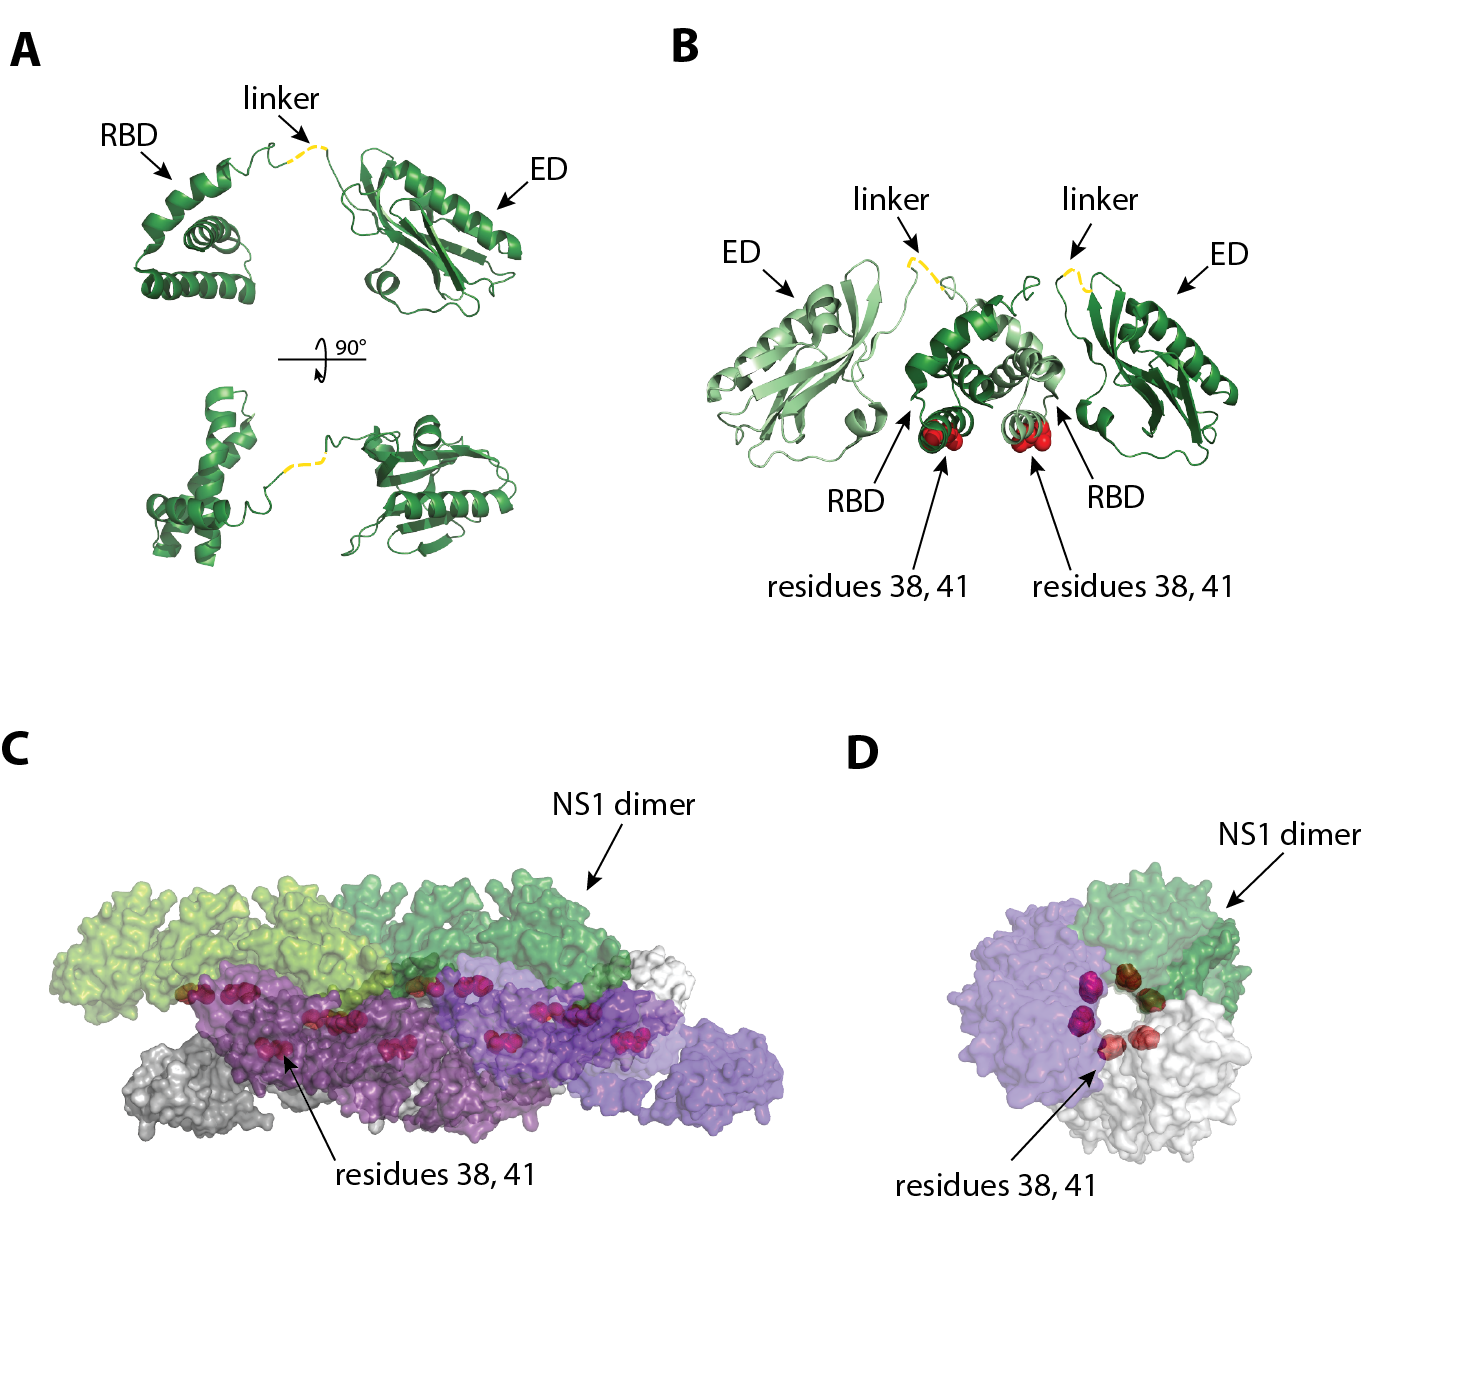
\includegraphics[width=\textwidth]{structure.png}}
			\caption{Crystal structure of H5N1 NS1 R38A, K41A mutant protein \parencite{Bornholdt2008}. (A) NS1 monomer; (B) NS1 dimer; (C,D) oligomerized NS1. The dimers are marked with distinct colors.} \label{fig:structure}
		\end{figure}
		
	
		\subsubsection{Inhibition of IFN signaling at pre-transcriptional level} \label{sec:pre-transcriptional}
		
		Inhibition of the interferon response is a function of NS1. The mechanisms behind this function have been extensively studied over the past two decades and according to the current paradigm NS1 subverts development of immune responses by counteracting PRR signaling, co- and post-transcriptional inhibiting of host gene expression and post-translationally inactivating  interferon-stimulated gene products \parencite{Ayllon2014}.	For this, the multi-functional NS1 targets numerous factors, which are discussed below. The mapped interactions of NS1 are schematically shown of Figure \ref{fig:NS1}.
		
		\begin{figure}[h]
			\centering
			\fbox{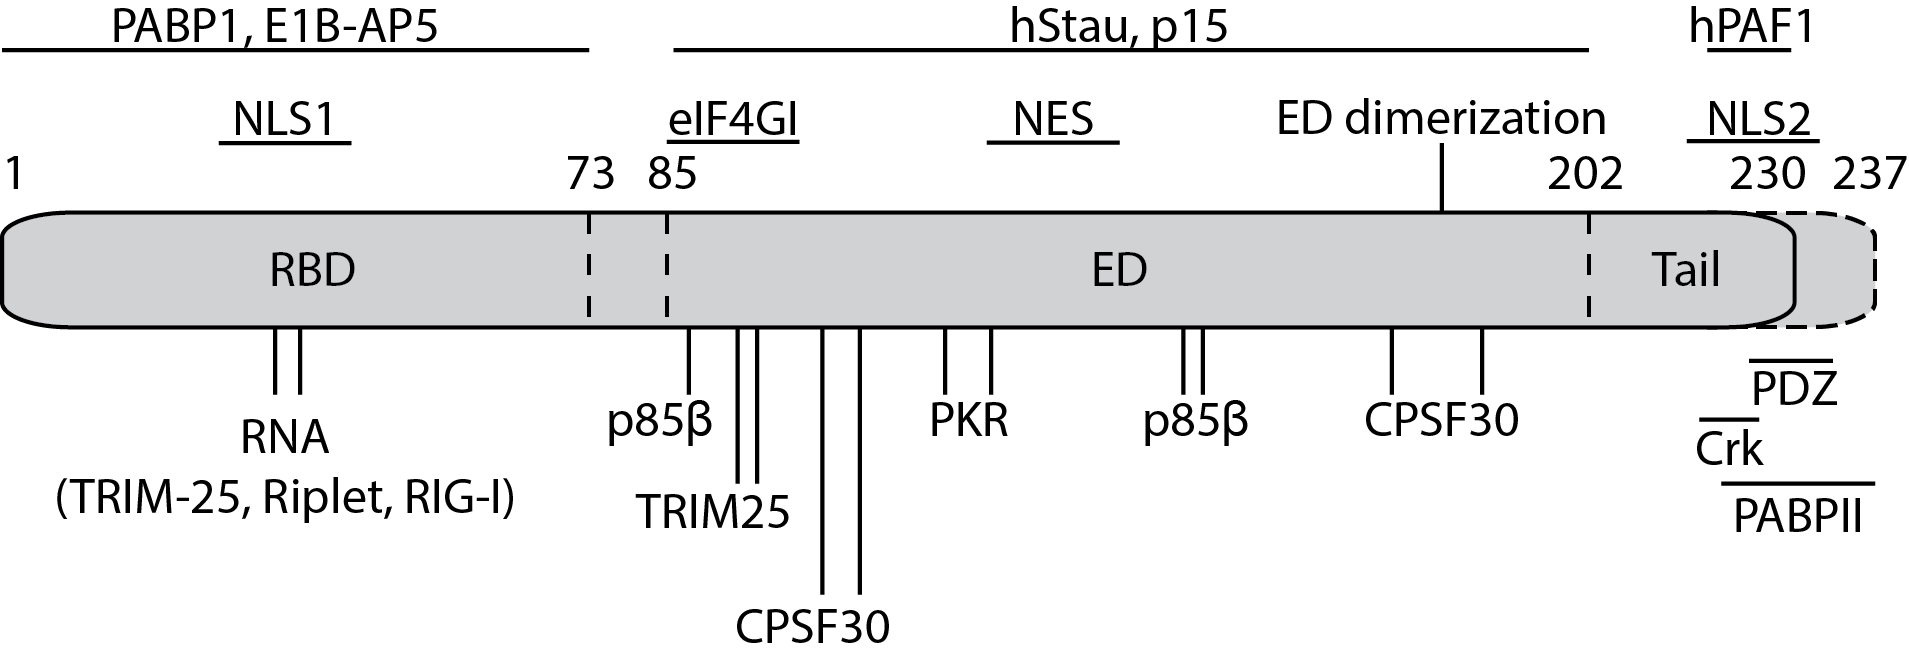
\includegraphics[width=\textwidth]{NS1.png}}
			\caption{Mapped interactions of NS1.} \label{fig:NS1}
		\end{figure}
				
		
		\gls{NS1} inhibits interferon signaling at the pre-transcriptional level by preventing activation and nuclear translocation of IRF3, AP-1, NFkB mainly by alleviating \gls{RIG-I} signaling \parencite{Talon2000, Ludwig2002, Wang2000, Geiss2002, Munir2012}. Multiple studies indicate that NS1 employs both its \gls{RBD} and \gls{ED} functions to subvert \gls{RIG-I} signaling at multiple steps \parencite{Haye2009, Ludwig2002, Tisoncik2011, Wang2000}. NS1 binds \gls{RIG-I}, although direct inhibitory effects of this interaction have not been reported yet \parencite{Opitz2007, Mibayashi2007a}. It also interacts with two indispensable \gls{RIG-I} regulators: TRIM25 and Riplet \parencite{Gack2009, Rajsbaum2012}. Interaction with TRIM25 requires E96, E97 residues within NS1 ED and RNA-binding residues R38, K41, although it is not clear whether the latter are involved in direct or RNA-mediated interaction or support suitable NS1 conformation \parencite{Gack2009}. Interaction with Riplet requires R38, K41 although again their exact roles in this interaction still need clarification \parencite{Rajsbaum2012}. The involvement of R38 and K41 residues in regulation of RIG-I has raised discussions of another possible mechanism of RIG-I inhibition by NS1 in which NS1 sequesters dsRNA, a known RIG-I inducer, thereby preventing activation of the RIG-I signaling axis. The role of NS1 RNA-binding in pre-transcriptional control   of immune responses, however, needs to be elucidated, because (i) influenza A does not seem to generate dsRNA during its replication \parencite{Wisskirchen2011} and (ii) the affinity of NS1 for dsRNA is much lower than that of RIG-I \parencite{Chien2004, Yin2007, Vela2012}.
		
		In addition to direct inhibition of RIG-I, NS1 has evolved several other ways to  effectively inhibit interferon induction at the transcriptional level. It subverts both canonical and non-canonical \gls{NFkB} pathways \parencite{Ruckle2012a} by preventing nuclear translocation of \gls{NFkB} via direct inhibition of alpha and beta subunits of \gls{IKK} \parencite{Gao2012}. \gls{NS1} impairs c-Jun and JNK signaling, preventing \gls{AP1}-regulated gene expression \parencite{Ludwig2002}. It also alleviates IFN response by inducing \gls{SOCS3}, a negative regulator of \gls{JAK}-STAT signaling \parencite{Pauli2008}. 
		
		\subsubsection{Inhibition of IFN signaling at post-transcriptional level}
		
		NS1 acts beyond pre-transcriptional level and controls development of antiviral responses also at post-transcriptionally by targeting pre-mRNA processing and nuclear export machinery of the host.
		The majority of cellular mRNAs produced by RNA pol II undergo cleavage of their 3' termini and subsequent addition of a \gls{polyA} which is required for their effective translation and also regulates their nuclear export \parencite{Vassalli1989, Zarkower1987, Huang1996}. Pre-mRNA cleavage and polyadenylation are catalyzed by \gls{CPSF}~--- a polyprotein complex formed by four subunits \parencite{Wilusz1990, Colgan1997}. NS1 binds \gls{CPSF}30, the smallest protein of subunit 4, thereby inhibiting the activity of the whole complex \parencite{Nemeroff1998}. The interaction between NS1 and \gls{CPSF}30 has been well characterized both biochemically and structurally and in the current model proposes interaction of NS1 ED with F2F3 zinc finger pocket of \gls{CPSF}30 \parencite{Noah2003, Twu2006, Kochs2007, Das2008}. Recent crystal studies suggest that ED dimerization is incompatible with \gls{CPSF}30 interaction \parencite{Aramini2011, Kerry2011}. Hydrophobic residues 184--188 within NS1 ED are essential for this interaction and mutation of G184 prevents NS1-CPSF complex formation \parencite{Das2008}. In addition, residues F103 and M106 facilitate NS1-CPSF30 complex formation \parencite{Kochs2007, Das2008}. Residues 223--237 within C-termini of some \gls{NS1} proteins comprise a site for interaction with \gls{PABP}II~--- another protein essential for effective polyadenylation \parencite{Li2001a}. Blocking cellular pre-mRNA processing via interactions with \gls{CPSF}30 and \gls{PABP}II provides several advantages for viral replication: (i) it prevents production of functional cellular mRNAs, including those involved in \gls{IFN} response; (ii) it prevents nuclear export of capped cellular mRNAs providing a pool of 5' caps to be ``snatched'' by viral polymerase \parencite{Nemeroff1998}; (iii) it does not inhibit production and export of viral mRNAs whose polyadenylation is independent of \gls{CPSF}30 \parencite{Plotch1977}. The residues involved in \gls{CPSF}30 binding are highly conserved among human influenza A NS1 proteins \parencite{Kochs2007, Das2008}. 
		
		Apart from non-specific post-transcriptional inhibition of cellular genes, NS1 of H3N2 subtype can specifically suppress a subset of cellular genes at transcriptional level. It acquired an \textsuperscript{226}ARSK\textsuperscript{229} sequence that mimics the histone H3 lysine 4 site \textsuperscript{226}ARTK\textsuperscript{229} thus gaining the ability to target  H3-interacting transcription elongation complex PAF1 and prevent its association with H3 \parencite{Marazzi2012}. PAF1 regulates RNA elongation and is important for pathogen-induced gene expression \parencite{Newey2009}. Thus NS1 specifically targets a PAF1-regulated gene subset that includes \gls{IFN} response genes \parencite{Marazzi2012}.
		
		NS1 also inhibits mRNA splicing by binding to the formed spliceosome and suppressing its catalytic activity \parencite{Lu1994, Qiu1995}. Interestingly, this effect is specific to host mRNAs. Although viral mRNAs recruit cellular spliceosome for their post-transcriptional processing, NS1 does not affect splicing of its own mRNA \parencite{Robb2010} and has little, if any, effect on M mRNA splicing \parencite{Salvatore2002, Robb2012}. The possible reason for such selectivity could be targeting of NS1 to specific recognition of motifs within viral mRNAs, which, however, is questionable, since no sequence specificity is so far known for NS1 RNA binding. Another possibility is recruitment of different spliceosomal factors to viral transcripts by viral polymerase \parencite{Fournier2014}.
		
		In addition to its direct effects on mRNA synthesis and processing, NS1 also inhibits nuclear export of cellular mRNAs. It specifically binds to nuclear pore complex components NXF1, p15, Rae1 and E1B-AP5, thus contributing to retention of cellular mRNAs in the nucleus \parencite{Satterly2007}. Importantly, inhibition of nuclear pore complex by NS1 does not attenuate viral replication, as export of viral RNAs relies on the alternative Crm1-mediated pathway \parencite{Neumann2000}.
		
		The combination of NS1 effects on host mRNAs production, processing and export contributes to host protein synthesis shut-off which is commonly observed during influenza A infection \parencite{Beloso1992}.
		
		\subsubsection{Direct inhibition of interferon-stimulated gene products} \label{sec:direct_inhibition}
		
		In addition to its control at pre-transcriptional, transcriptional and post-transcriptional level, NS1 antagonizes \gls{IFN} responses by directly targeting \gls{PKR} and \gls{OAS}. 
		
		Influenza A mRNAs are structurally indistinguishable from cellular mRNA and hence production of viral proteins requires functional cap-dependent translation. For this, the virus prevents activation of the negative translational regulator \gls{PKR}  \parencite{Katze1986, Katze1988}. \gls{PKR} inhibition is to a large extent a function of \gls{NS1}, as viruses lacking functional \gls{NS1} can only replicate in the absence of \gls{PKR} \parencite{Bergmann2000a}. \gls{NS1} was proposed to prevent activation of \gls{PKR} by binding to dsRNA and thus sequestering it away from \gls{PKR} \parencite{Lu1995}. Such regulation, however, seems unlikely for several reasons: (i) while \gls{PKR} senses dsRNA in the cytoplasm, the site of influenza A replication is the nucleus, and thus the presence of virus replication intermediates in the cellular cytoplasm is unlikely \parencite{Jackson1982}, (ii) viral genomes are exported to the cytoplasm as \gls{vRNP}s, and thus base-paired regions of \gls{vRNA} are likely to be inaccessible for \gls{PKR} \parencite{Coloma2009}, (iii) the affinity of \gls{NS1} for dsRNA is much lower than that of \gls{PKR} \parencite{Chien2004, Husain2012}, and (iv) dsRNA binding function of \gls{NS1} is not required for \gls{PKR} inhibition \parencite{Li2006}. \gls{NS1} has been shown to form a complex with \gls{PKR} which appears to be inhibitory for \gls{PKR} activation \parencite{Tan1998, Li2006}. It has been shown that residues 123--127 within \gls{NS1} are required for interaction with \gls{PKR} and its inhibition \parencite{Min2007}.	
				
		Inhibition of \gls{OAS}/\gls{RNAseL} pathway is also a function of \gls{NS1}. So far only one study has described the putative mechanism of \gls{NS1} control over the \gls{OAS}/\gls{RNAseL} pathway which presumes that dsRNA binding by NS1 is required for sequestration of dsRNA away from \gls{OAS} \parencite{Min2006}. This observation is supported by low affinity of \gls{OAS} to dsRNA \parencite{Hartmann2003}, however, the abundancy of influenza-generated dsRNA in cell cytoplasm still remains an open question.
		
		\subsubsection{Other pro-viral functions of NS1}
		
		In addition to its critical role in control of innate immune responses, NS1 targets a number of other cellular factors to facilitate virus replication. These additional pro-viral functions of NS1 include regulation of production of viral RNA and protein synthesis, control of apoptosis and modulation of cell signaling.
		
		Influenza A virus RNA production occurs in two phases: early, when \gls{NS1} and \gls{NP} vRNAs are preferentially synthesized, and late, when all eight segments are produced in equimolar quantities \parencite{Shapiro1987, Skehel1973}. This temporal regulation of vRNAs production has been shown to require functional \gls{NS1} \parencite{Falcon2004} and is linked to residues 123 and 124 within its ED \parencite{Min2007}. Although these residues overlap with the \gls{PKR} binding site on NS1, NS1 regulates vRNA independently of its interaction with PKR, which has been proven using PKR deficient mice \parencite{Min2007}. NS1 through an as yet unknown mechanism also specifically regulates production of HA vRNA \parencite{Maamary2012}. The regulation of vRNAs production by NS1 is likely linked to its interaction with \gls{vRNP}s which disrupts inhibitory binding of cellular helicase DDX21 to PB1 \parencite{Marion1997a, Chen2014}.
		
		\gls{NS1} has been also discussed as a factor that regulates protein synthesis in infected cells. As viral mRNAs contain \gls{5meG} ``cap'' and 3' \gls{polyA}, they are structurally indistinguishable from cellular mRNAs and require the same subset of translation factors \parencite{Poch1989, Poon1999}. The bottleneck of the complex translation process is its initiation which requires coordinated assembly translation factors and 43S pre-initiation complex on mRNA followed by start codon scanning and ribosome assembly \parencite{Pestova2001}. In addition to the prevention of \gls{eIF2a} inhibition \gls{PKR} described in section \ref{sec:direct_inhibition}, \gls{NS1} contributes to translational control by direct interactions with translation initiation factors. Thus, fragment 1--81 has been shown to bind the \gls{eIF4GI} via protein-protein interactions and is supposed to facilitate recruitment of this factor onto viral mRNAs \parencite{Aragon2000}. In addition, it interacts with \gls{PABP}I, another factor essential for translation initiation \parencite{Burgui2003}. The proposed mechanism of translational regulation by \gls{NS1} suggests preferential recruitment of translation initiation factors on viral mRNAs due to specific recognition of their 5' \gls{UTR} by NS1 \parencite{DelaLuna1995}. Such a mechanism, however, is in controversy with the very low affinity of NS1 to ssRNA and with its proposed nonsequence-specific binding to RNA \parencite{Hatada1992} and requires further description of NS1 interactions with translation factors and/or search for possible specificity of NS1 towards viral mRNAs.
	
		Influenza A infection induces transient activation of \gls{PI3K} and its downstream effector Akt signaling during virus attachment and prolonged activation several hours later due to \gls{NS1} activity \parencite{Ehrhardt2006, Ehrhardt2009}. \gls{NS1} forms the heterotrimeric complex with regulatory (p85) and catalytic (p110) subunits of \gls{PI3K}, altering their respective positions and resulting in \gls{PI3K}/Akt signaling activation \parencite{Hale2008d, Hale2010c}. The interaction between \gls{NS1} and p85 is dependent on the \textsuperscript{164}PxxP1\textsuperscript{167} \gls{SH3} motif and a conservative tyrosine 89 within \gls{NS1} \gls{ED} \parencite{Hale2006, Shin2007a, Shin2007}. As \gls{PI3K}/Akt signaling inhibits apoptosis, its activation by \gls{NS1} was initially regarded as a mechanism to prevent premature cell death and secure viral replication \parencite{Ehrhardt2007, Zhirnov2007}. However, p85-binding deficient \gls{NS1} also exibits anti-apoptotic activity indicating possible redundancy in NS1 approaches to control apoptosis \parencite{Jackson2010a}.
		
		In addition to the \gls{PI3K}/Akt branch, \gls{NS1} also controls the \gls{JNK} branch of apoptosis. This control is realized through binding of \gls{SH3} domains present in some \gls{NS1} subtypes to cellular adapter proteins Crk and Crk-like \parencite{Heikkinen2008, Hrincius2010}.
		
		An additional way by which \gls{NS1} protects infected cells from apoptosis could be its ability to bind to PDZ-domain containing proteins \parencite{Liu2010}. The C-terminus of 230 \gls{aa} long avian \gls{NS1}s can contain a PDZ binding motif ESEV/EPEV, which mediates interaction with PDZ-domain containing proteins \parencite{Golebiewski2011}. In addition to apoptosis regulation, PDZ binding may provide control over formation of cellular junctions and establishment of cell polarity, although these possibilities, as well as overall effect of PDZ-binding on influenza A virulence are yet to be investigated \parencite{Jackson2010, Zielecki2010, Javier2011}.
		
		
		
		
		%NS1 inhibits not only development of innate immune responses to influenza A, but also prevents effective establishment of adaptive immunity, inhibiting antigen presentation pathways \parencite{Tisoncik2011}
				
	
		%NS1 was discovered as anti-interferon protein, then it was found that functional NS1 is necessary for virus growth in immune competent systems and viruses with truncated or delNS1 are not growing in normal cells, but grow in vero and are lethal in stat-/- mice. The role of NS1 is established and it is to secure viral replication, but the strategy can be unclear. This is because its multifunctionality.
		
		%NS1 temperature sensitive mutants revealed also a possible role of NS1 in late steps of viral replication cycle \parencite{Garaigorta2005}.
		
		%RK/AA virus in TRIM25 -/- cells induces IFN (although not high levels) -- there are other that RIG-I pathways that induce IFN (Gack 2009)
		
		\subsubsection{NS1 diversity}
		
		NS1 contributes to influenza A variability by displaying a substantial number of sequence, length, structure, modification and functional polymorphisms. Initial studies of sequence similarity revealed two groups of \gls{NS1} proteins designated alleles A and B \parencite{Scholtissek1980}. Allele A \gls{NS1}s have been found in avian strains, as well as mammalian, whereas allele B appears to be exclusively avian indicating the contribution of NS1 to host-specificity \parencite{Treanor1989, Ludwig1991}. The percentage of sequence identity is over 90 \% within alleles, but between alleles it is below 70 \% \parencite{Scholtissek1980}.
		
		Structural polymorphisms of \gls{NS1} are mainly dependent on the length of inter-domain linker. A recent study has shown that the linker length and residue 71 determine the preference of \gls{RBD} orientation towards \gls{ED} and provide structural basis for strain-dependent \gls{NS1} functions \parencite{Carrillo2014}. Interestingly, whereas the inter-domain linker is 12 amino acid long in the majority of \gls{NS1}s, its length in highly pathogenic avian influenza A viruses is only 7 amino acids, indicating that although there are no known interaction motifs within the linker, it still can determine virulence \parencite{Long2008}.
		
		Although functional \gls{NS1} is required for replication in immune-competent systems \parencite{Garcia-Sastre1998, Donelan2003}, \gls{NS1}s from different subtypes may vary in their ability to modulate certain cellular responses. For example, although different \gls{NS1}s are able to bind components of the \gls{RIG-I} pathway, the extent to which they inhibit \gls{RIG-I} signaling varies and some H1N1, H2N2 and human H3N2 viruses fail to pre-transcriptionally block \gls{IFN} induction \parencite{Kochs2007, Haye2009, Munir2011a, Munir2012}. These viruses compensate for their inefficiency in pre-transcriptional control with strong \gls{CPSF}30 binding, whereas the mouse-adapted PR8 strain as well as the pandemic H1N1 acquired mutations that prevent interactions with \gls{CPSF}30 \parencite{Kochs2007, Hale2010d}. Human and avian \gls{NS1} proteins also markedly differ in their ability to modulate signaling pathways: instead of functional PDZ-binding motifs ESEV/EPEV found in avian strains, human NS1s contain RSKV/RSEV motifs that can not interact with PDZ-domain containing proteins \parencite{Liu2010}. Furthermore, interaction with CRK and CRK-like protein adapters is also a characteristic of avian strains and the 1918 pandemic influenza A virus which contain SH3-binding motif \parencite{Heikkinen2008}.
		
		Naturally occurring \gls{NS1} proteins vary in length due to C-terminal truncations and extensions that arise via appearance or loss of nonsense codons \parencite{Parvin1983}. Although selective pressure maintains avian and avian-originated human \gls{NS1} at 230 aa and human pH1N1 at 219 aa, the appearance of truncated isolates is not uncommon \parencite{Suarez1998, Lakspere2014}. The attempts to address the effects of \gls{NS1} C-terminal truncations on viral pathogenicity brought controversial results and the significance of these truncations is still unclear \parencite{Hale2010e, Tu2011a}. The relatively short NS1 C-terminus can accommodate, lose or acquire a number of binding motifs and modification sites that can mediate virus-host interactions, including PDZ- and Crk/CrkL-binding sites \parencite{Heikkinen2008, Liu2010}, histone mimic motif \parencite{Marazzi2012}, \gls{PABP}II  \parencite{Li2001a}, nuclear and nucleolar localization sites \parencite{Melen2012}, phosphorylation \parencite{Hsiang2012} and \gls{ISG}ylation sites \parencite{Hsiang2009} and therefore addressing the role of NS1 C-terminal polymorphisms could be beneficial for understanding viral evolution and pathogenicity.
		
		
		
		
		%functions of NS1 may be specific to cell type or to virus subtype
		%many motifs for interactions 
		%some motifs are conserved, whereas some are variable
		%NS1 can loose/acquire some during evolution
		
		%Responses can be dependent of viral subtype -- MyD88 is not required for H1N1, but is required for H3N2 (Seo2010, LeGoffic2006)
		
		%Kochs2007 -- some NS1 inhibit IRF3 and IFNB signaling, 	strain-specific differences
		
		%Haye2009 -- in DCs, TX 1-126 cannot block IFN response, less late viral protein expression, Tx 1-99 and 1-126 have more phospho-IRF3, DCs infected with NS1 mutants have upregulation of IFN I responses, ISGs adn, proinflammatory genes. They are better in stimulating adaptive immune, responses WT human isolate (Tx) is better inhibitor than PR8
		
		%Zhang2010a	heterologous expression of SH3beta inhibits IAV strain-specifically
		
				
		%Regulation of interferon-β by MAGI-1 and its interaction with influenza A virus NS1 protein with ESEV PBM.		Kumar M, Liu H, Rice AP.
		
		%Suarez and Perdue, 1998 C-term length
		
		%The deletion of residues 80–84 found in recent H5N1 strains is
		%implicated in cytokine resistance but not virulence9,11
		%9. Seo, S.H., Hoffmann, E. & Webster, R.G. Nat. Med. 8, 950–954 (2002). 10. Seo, S.H., Hoffmann, E. & Webster, R.G. Virus Res. 103, 107–113 (2004). 11.Lipatov,A.S. et al. J. Gen. Virol. 86, 1121–1130 (2005).
		%Li, K. S. et al. Genesis of a highly pathogenic and potentially pandemic H5N1 influenza virus in eastern Asia. Nature 430, 209–213 (2004)
		
		% % % % % % % % % % % RESULTS AND DISCUSSION % % % % % %
		%\subsubsection{NS1 as a therapeutic target -- this goes to discussion}
		
		%\textit{Discuss the importance of NS1 for successful viral replication, possibly (?) delNS1 vaccine and attempts to develop drugs targeting NS1. Finish with stressing the importance of thorough understanding of IAV-host cell intercations for development of novel treatment options and IAV surveilance.}
		
		
		%In results about translation cite Marc 2013 rna specific binding and wang 2014 non-specific regulation of translation
		
		%Marc -- AGCAAAAG motif in their 5 prime UTR
		%Kash2002 -- AGGGU motif 5 prime (NS1 and NP)
		
		%NS1 C-terminus contains a number of positive selection sites --- Xu2014